\part{Electrones, transporte electrónico}

\chapter{Modelo de Drude}

A lo largo del bloque se estudiarán diversos modelos. Comenzamos con
el modelo de Drude y el de Sommerfield, que suponen
\begin{itemize}
\item Electrones libres (no hay interacción con el potencial de la red).
\item No hay interacción electrón-electrón.
\end{itemize}
Modelos más complicados, como los electrones Bloch, liberan la primera
restricción. Prescindir de la segunda excede gratamente el nivel de este curso.

El modelo de Drude fue formulado por P. Drude en el año 1900, cuatro


años después del descubrimiento del electrón por J. J. Thompson. La
base es la teoría cinética clásica.

Estimamos la densidad electrónica y con ella el radio ``efectivo'' de
los electrones:
\begin{equation}
  \underbrace{n}_{\sim 10^{22} \text{cm}^{-3}} \sim
  \frac{1}{\frac{4}{3}\pi r_s^3} \rightarrow r_s \sim 2.5 a_0
\end{equation}
Utilizo varias hipótesis:
\begin{itemize}
\item Los electrones son libres y no interactúan entre ellos. La
  aproximación más restrictiva es la primera (no interacción con la red).
\item . El mecanismo es irrelevante,
  Drude propuso que se producía con los iones de la red.
\item Realizamos una aproximación de tiempo de relajación, donde
  $\tau \sim \text{cte.}$ es el tiempo medio entre colisiones. $\tau$
  es independiente de la posición o velocidad.
\item El equilibrio térmico de los electrones se alcanza a base de
  colisiones con la red, los electrones sufren procesos de scattering
  instantáneos que les producen cambios en la velocidad. La velocidad tras la colisión depende de la temperatura local,
  vía $\frac{1}{2}mv^2 \sim \frac{3}{2}\kb  T$.
\end{itemize}

Tratamos de resolver la conducción eléctrica con el modelo.
\section{Conducción eléctrica}
\emph{\small{Nota: la constante \emph{e} es positiva}}.


Si el campo eléctrico es nulo, el promedio de la velocidad electrónica
es nulo, y por tanto $\mathbf{J} = -neo\langle \mathbf{v}\rangle =
0$. Aplicamos un campo $\mathbf{E}$ no nulo constante, en $t=0$ se
produce el primer choque y el electrón en cuestión obtiene una
velocidad $\mathbf{v}_0$. Mientras no choque, irá incrementando su
velocidad por efecto del campo eléctrico:
\begin{equation}
\begin{split}
  \mathbf{v}(t) &= \mathbf{v}_0 - \frac{e \mathbf{E} t}{m} \\
  \langle \mathbf{v}\rangle &= \underbrace{\langle
                              \mathbf{v}_0\rangle}_{=0} - \frac{e}{m}
                              \mathbf{E} \underbrace{\langle t
                              \rangle}_{=\tau} = \frac{-e}{m} \mathbf{E}\tau
\end{split}
\end{equation}
donde $\langle \mathbf{v}_0\rangle$ es nulo porque las direcciones de
los electrones tras la colisión son aleatorias. Para la densidad de
corriente tenemos:
\begin{equation}
  \mathbf{J} = -ne \left( \frac{-e \mathbf{E}\tau}{m} \right) =
  \frac{n e^2 \tau}{m} \mathbf{E} = \sigma \mathbf{E} \tag{Ohm's law}
\end{equation}
con $\sigma = \rho^{-1} = \frac{n e^2 \tau}{m}$. Como consecuencia,
$\tau=\tau(T) \rightarrow \sigma = \sigma(T)$. Valores típicos de
$\tau$ son  \SI{27}{\femto\second} a \SI{273}{\kelvin}  y \SI{210}{\femto\second} a \SI{77}{\kelvin}.

El recorrido libre medio es $l = v_0 \tau$, con $v_0$ estimable como
\begin{equation}
  \frac{1}{2} m v_0^2 = \frac{3}{2} \kb  T \ \rightarrow \ v_0 = \left(
    \frac{3\kb T}{M} \right)^\frac{1}{2}
  \stackrel{\SI{273}{\kelvin}}{\sim} \SI{1e7}{\centi\metre\per\second}
\end{equation}
Por tanto $l \sim 5 \AA$, los electrones casi no salen de la celda
unidad sin chocar.

\section{Momento electrónico}
La ley de conservación del momento nos dice que
\begin{equation}
\begin{split}
  \mathbf{p}(t + \text{d}t) &= [\mathbf{p}(t) +
  \mathbf{F}(t)\text{d}t]\left( 1- \frac{\text{d}t}{\tau} \right) \sim
  \\ &\sim \mathbf{p}(t) - \mathbf{p}(t)\frac{\text{d}t}{2} + \mathbf{F}(t)\text{d}t
\end{split}
\end{equation}
donde $\mathbf{F}$ es una fuerza genérica y
$\left( 1- \frac{\text{d}t}{\tau} \right)$ es la probabilidad de no
colisión. El diferencial del momento será
$\text{d}\mathbf{p} = \mathbf{p}(t+\text{d}t) - \mathbf{p}(t)$,
desarrollándolo con el resultado anterior para
$\mathbf{p}(t+\text{d}t)$ obtenemos:
\begin{equation}
\begin{split}
  \text{d}\mathbf{p} &= \underbrace{+\mathbf{p}(t) -
\mathbf{p}(t)\frac{\text{d}t}{2} + \mathbf{F}(t)
\text{d}t}_{\mathbf{p}(t + \text{d}t)} - \mathbf{p}(t) = \\ &=
\mathbf{p}(t)\frac{\text{d}t}{2} + \mathbf{F}(t) \text{d}t
\end{split}
\end{equation}

Reordenando llegamos a
\begin{equation}
  \frac{\text{d}\mathbf{p}}{\text{d}t} = \frac{-\mathbf{p}(t)}{\tau} + \mathbf{F}(t)
\end{equation}
El modelo de Drude supone por tanto que si no hay una fuerza externa
se vuelve al equilibrio de forma exponencial, según el tiempo de
relajación ($\mathbf{p}(t) = \mathbf{p}_0 e^{-t/\tau}$).

\section{Efecto Hall, magnetoresistencia}
Si la fuerza externa es causada por un campo magnético, se tiene por
la ley de Lorentz que
\begin{equation}
  \mathbf{F}(t) = -e \mathbf{E} - e \mathbf{v}\times \mathbf{B} = -e
                  \mathbf{E} - \frac{e}{m} \mathbf{p}\times \mathbf{B}
\end{equation}
y por tanto
\begin{equation}
\begin{split}
  \frac{\text{d}\mathbf{p}}{\text{d}t} &= \frac{-\mathbf{p}}{\tau}-
                                         \mathbf{F} = \\
                                       &= \frac{-\mathbf{p}}{\tau} - e
                                         \mathbf{E} - \frac{e}{m}
                                         \mathbf{p}\times \mathbf{B}
\end{split}
\end{equation}
Inyectamos una corriente en la dirección
$\hat x$, sobre una placa fina situada en el plano
$XY$. En $\hat z$ se aplica un campo magnético.

En condiciones estacionarias tenemos:
\begin{equation}
\begin{split}
  \frac{\text{d}p_x}{\text{d}t} &= \frac{-p_x}{\tau}-e E_x -
                                  \frac{e}{m}p_y B = 0 \\
  \frac{\text{d}p_y}{\text{d}t} &= \frac{-p_y}{\tau}-e E_y +
                                  \frac{e}{m}p_x B = 0
\end{split}
\end{equation}

La corriente inyectada en $\hat x$ será de la forma $\mathbf{J} = - n
e \mathbf{v} = - \frac{ne}{m} \mathbf{p}, \ \mathbf{J} \parallel \hat x$.
Suponemos que $p_y$ es por tanto prácticamente nulo. Sustituyendo los
nuevos valores para los momentos ($p_y = 0, \ p_x = \frac{-j_x
  m}{ne}$) en la ecuación para $\frac{\text{d}p_x}{\text{d}t}$, se obtiene
\begin{equation}
  \frac{m}{ne\tau}j_x - eE_x = 0 \ \rightarrow \sigma_x =
  \frac{ne^2\tau}{m} \neq f(B)
\end{equation}
Obtenemos el primer fallo de este modelo, pues la conductividad sí que
depende del campo magnético de manera tenue (a este fenómeno se le
denomina \emph{magnetorresistencia}). Sustituyendo en la
ecuación de $\frac{\text{d}p_y}{\text{d}t}$:
\begin{equation}
  E_y = \frac{1}{m}p_x B = \frac{-1}{ne}Bj_x
\end{equation}
Obtenemos una predicción de campo en $\hat y$, el denominado
\emph{efecto Hall}. Va gobernado por un coeficiente $R_H$ tal que
\begin{equation}
  \frac{E_y}{j_x B} = \frac{-1}{ne} = R_H
\end{equation}
Con mediciones del efecto Hall puedo calcular $n$, y si ya lo conozco
$B$. Es el fundamento de las sondas magnéticas por efecto Hall.

El modelo de Drude predice que $R_H < 0$, y que no es función ni de la
temperatura ni del campo. No obstante, sí que es función de dichos
parámetros, y a veces incluso es mayor que cero.

\section{Conductividad AC}
Sabemos que
$\frac{\text{d}\mathbf{p}(t)}{\text{d}t} = -
\frac{\mathbf{p}(t)}{\tau} + \mathbf{F}(t)$,
investiguemos el efecto de un
$\mathbf{E} = \mathbf{E}(t) = \mathbf{E}(\omega) e^{-i\omega t}$. Si
busco soluciones de la forma
$\mathbf{p}(t) = \mathbf{p}(\omega) e^{-i\omega t}$ obtengo tras
sustituir:
\begin{equation}
  \mathbf{p}(\omega) = \frac{-e \mathbf{E}(\omega)}{\frac{1}{\tau}- i\omega}
\end{equation}
por tanto, como $\mathbf{J}(t) = -n e \mathbf{v}(t) = \frac{-ne}{m}
\mathbf{p}(t)$,
\begin{equation}
\begin{split}
  \mathbf{J}(\omega) &= \frac{\frac{ne^2}{m}}{\frac{1}{\tau}-i\omega}
  \mathbf{E}(\omega) = \frac{\frac{ne^2\tau}{m}}{1-i\omega \tau}
  \mathbf{E}(\omega) = \\ &= \sigma(\omega) \mathbf{E}(\omega)
\end{split}
\end{equation}
donde $\sigma(\omega) = \frac{\sigma_0}{1-i\omega \tau}$, con
$\sigma_0 = \frac{ne^2\tau}{m}$. A $\omega = 0$ recupero los
resultados de DC.

Utilizando las ecuaciones de Maxwell (concretamente que $\nabla^2
\mathbf{E} + \frac{\omega^2}{c^2} \epsilon(\omega) \mathbf{E} = 0$), puedo derivar la constante
dieléctrica del medio. Obtengo
\begin{equation}
  \epsilon(\omega) = 1 + \frac{i \sigma(\omega)}{\epsilon_0 \omega}
  \stackrel{\omega\tau \gg 1}{\sim} 1 - \frac{\omega_p^2}{\omega^2}
\end{equation}
donde a $\omega_p = \left( \frac{\sigma_0}{\epsilon_0 \tau}
\right)^{\frac{1}{2}} = \left( \frac{ne^2}{m\epsilon_0}
\right)^{\frac{1}{2}}$ se le denota \emph{frecuencia del
  plasma}. Según el valor de $\omega_p$ tenemos dos regímenes para una
onda electromagnética de frecuencia $\omega$:
\begin{itemize}
\item Si $ \omega < \omega_p$ la constante dieléctrica es negativa y
  real; $\kappa^2 = \frac{\omega^2}{c^2} \varepsilon(\omega)$ es imaginaria y las ondas electromagnéticas decaen de
  forma exponencial dentro del metal, haciéndolo opaco.
\item $\omega > \omega_p$ implica una $\varepsilon(\omega)$
real y positiva, y por tanto $\kappa(\omega)$ es real. La onda puede
atravesar el metal sin atenuación; el metal es transparente a la onda electromagnética.
\end{itemize}

El valor de $\omega_p$ es de aproximadamente \SI{1e15}{\hertz}, lo
que nos da ondas electromagnéticas de unos \SI{300}{\nano\metre} (UV cercano).


\section{Propiedades térmicas}
La teoría cinética elemental (los cálculos son similares a los de los
fonones, sección \ref{sec:tce}) nos da
$\mathbf{J}_Q = - \kappa \nabla T$, con
$\kappa = \frac{1}{3}c_v v^2 \tau$ (con los parámetros electrónicos en
lugar de los de los fonones). Hallando el calor específico
($\frac{1}{2}mv^2 = \frac{3}{2}\kb  T \rightarrow c_v = \frac{3}{2}n
\kb  $) y con la fórmula obtenida para la conductividad eléctrica
($\sigma = \frac{ne^2 \tau}{m}$) podemos obtener la ley de
\emph{Wiedemann-Franz} (1853):
\begin{equation}
  \frac{\kappa}{\sigma} = \cdots = LT\propto T
\end{equation}
La teoría de Drude reproduce por tanto correctamente esta ley
experimentalmente comprobada, pero la constante de proporcionalidad
$L$ es la mitad del valor experimental.

La realidad es que el resultado es una afortunada coincidencia, ya que
$c_v$ difiere del valor experimental en un factor $\frac{1}{100}$ y
$v$ en un factor $100$, cancelándose los errores.

\section{Efecto Seebeck}
El \emph{efecto Seebeck} se basa en la aparición de un voltaje al
aplicar gradientes de temperatura y viceversa. Hay una explicación
detallada en el Callen, capítulo ``Irreversible Thermodinamics''.

De manera precisa:
\begin{equation}
  \Delta T \rightarrow \mathbf{E} = Q \Delta T
\end{equation}
A la constante $Q$ se la denota \emph{thermopower}. Para deducirla,
vemos las contribuciones a la velocidad de los electrones por el
gradiente térmico y el eléctrico:
\begin{description}
\item[Gradiente térmico] La velocidad media por el $\Delta T$ es
\begin{equation}
  v_Q = \frac{1}{2}[v(x-v\tau) - v(x+v\tau)] \sim - v\tau
  \frac{\text{d}v}{\text{d}x} = - \frac{1}{2}\tau
  \frac{\text{d}(v^2)}{\text{d}x} = -\frac{1}{2}\tau \frac{\text{d}(v^2)}{\text{d}T}\frac{\text{d}T}{dx}
\end{equation}
Por tanto $v_Q = \frac{-1}{2}\tau \frac{\text{d}v^2}{\text{d}T} \nabla
T$.
\item[Campo eléctrico] El campo eléctrico genera una velocidad media
  $v_E = - \frac{e E \tau}{m}$.
\end{description}
En estado estacionario, ambas deben ser iguales. Obtenemos:
\begin{equation}
  \mathbf{E} = \frac{-m}{6e} \frac{\text{d}v^2}{\text{d}T} \nabla T =
  Q \nabla T
\end{equation}
El modelo de Drude nos predice por tanto un \emph{thermopower} de
valor
\begin{equation}
  Q = \frac{-m}{6e} \left[ \frac{2}{m}
    \frac{\text{d}}{\text{d}T}\left( \frac{1}{2}mv^2 \right) \right]
  = \frac{-c_v}{3ne} = \cdots
\end{equation}
utilizando como calor específico $\frac{3}{2}n \kb $,
\begin{equation}
  \cdots = \frac{-\kb }{2e} = \text{cte.} \sim -43 \ \mu\text{V/K}
\end{equation}
Experimentalmente, se comprueba que no es constante y ronda el
$\mu \text{V/K}$. Además, puede ser positivo para algunos metales. El
error en magnitud (un factor cien) es explicable por la pobre
estimación de $c_v$ que ya se comentó en la sección de propiedades
térmicas.

\chapter{Modelo de Sommerfield}
Para mejorar el modelo de Drude podemos utilizar la estadística de
Fermi-Dirac en lugar de la de Boltzmann. Aproximamos el metal a un gas
de Fermi a temperatura nula (la aproximación es razonable por lo
elevado de las temperaturas de Fermi, recordar los apuntes de
termodinámica).

Suponemos electrones libres (usaremos una aproximación
monoelectrónica), con función de onda $\psi$ definida como
\begin{equation}
  \psi _\mathbf{k} (\mathbf{r}) = \frac{1}{V} e^{i \mathbf{k}\mathbf{r}}
\end{equation}
Utilizamos condiciones periódicas, lo que nos impone
\begin{equation}
  k_i = \frac{2\pi n_i}{L_i}, \ \
  \begin{cases}
    &i = \{x,y,z\} \\
    &n_i \in \mathbb{Z}
  \end{cases}
\end{equation}
Un valor de $\mathbf{k} = \{k_x,k_y,k_z\}$ ocupa un volumen
$\frac{(2\pi)^3}{V}$ (fig. \ref{fig:sommk}), si intento acomodar $N$ electrones con
degeneración $2s+1$ ($s = \frac{1}{2}$) obtengo el vector de ondas de Fermi:
\begin{equation}
  N = 2 \cdot \frac{\frac{4}{3}\pi k_F^3}{\frac{(2\pi)^3}{V}} \
  \rightarrow \ k_F = \left( \frac{3\pi^2N}{V} \right)^\frac{1}{3} = \left( {3\pi^2n}\right)^\frac{1}{3}
\end{equation}
Podemos deducir los demás parámetros de Fermi con la $k_F$:
\begin{description}
\item[Nivel de Fermi] $ \varepsilon_F = \frac{\hbar^2 k_F^2}{2m}=
  \frac{\hbar^2}{2m}(3\pi^2 n)^{2/3}$
\item[Velocidad de Fermi] $v_F = \frac{\hbar k_F}{m} = \frac{\hbar}{m}$
\item[Temperatura de Fermi] $\varepsilon_F = \kb  T_F $, por lo que $T_F =
  \frac{\hbar^2}{2m \kb }(3\pi^2 n)^{2/3}$
\end{description}


\begin{figure}
  \centering
  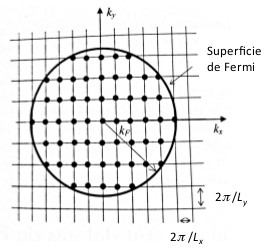
\includegraphics[width=0.6\textwidth]{figures/sommk.png}
  \caption{Cada $k$ está separada en la red recíproca por
    aproximadamente $\frac{2\pi}{L_i}$}
  \label{fig:sommk}
\end{figure}

Si no estoy a temperatura nula, la distribución de estados es la
función de distribución de Fermi ya conocida:
\begin{equation}
  f(\varepsilon,T) = \frac{1}{\exp \left(\frac{\varepsilon-\mu}{\kb  T}\right)+1}
\end{equation}
La función de distribución es similar a un escalón, pero con el salto
suavizado y de anchura aproximada $\kb  T$. El escalón se produce en
$\varepsilon_F$. Si $\varepsilon-\mu
\gg \kb  T$ recuperamos la función de distribución de Boltzmann.

El potencial químico puede aproximarse con la expansión de
Sommerfield:
\begin{equation}
  \label{eq:somm}
  \mu(T) \sim \varepsilon_F - \frac{\pi^2}{6} (\kb  T)^2
  \frac{D'(\varepsilon_F)}{D(\varepsilon_F)} = \varepsilon_F \left[ 1-
    \frac{\pi^2}{12} \left( \frac{\kb  T}{\varepsilon_F} \right) ^{\frac{1}{2}}\right]
\end{equation}

La densidad de estados es proporcional a $\varepsilon^\frac{1}{2}$, ya
que $N \propto \varepsilon^{\frac{3}{2}}$, y por tanto
$\frac{\text{d}N}{N} = \frac{3}{2}
\frac{\text{d}\varepsilon}{\varepsilon}$ obteniendo
\begin{equation}
  D(\varepsilon) = \frac{\text{d}N}{\text{d}\varepsilon} =
  \frac{3}{2}\frac{N}{\varepsilon} \propto \frac{\varepsilon^{\frac{3}{2}}}{\varepsilon} \propto \varepsilon ^ \frac{1}{2}
\end{equation}
No es necesario acotarla como en la estadística de Debye, ya que hay
un corte natural de la energía en $\varepsilon_F$.

\section{Calor específico}
La energía es
\begin{equation}
  U(T) = \int_\mathbb{R^+} \varepsilon f(\varepsilon, T)
  D(\varepsilon) \text{d} \varepsilon
\end{equation}
Observando la forma funcional (fig. \ref{fig:usomm}), la integral es fácilmente aproximable:
\begin{equation}
  \begin{split}
    U(T) &\sim \underbrace{N \frac{\kb 
        T}{\varepsilon_F}}_{\text{fraction of e\textsuperscript{-}
        passing}} \cdot \underbrace{\kb 
      T}_{\text{energy increment}} = \\
    &= \frac{N\kb ^2}{\varepsilon_F}T^2 \propto T^2
  \end{split}
\end{equation}
\begin{figure}
  \centering
  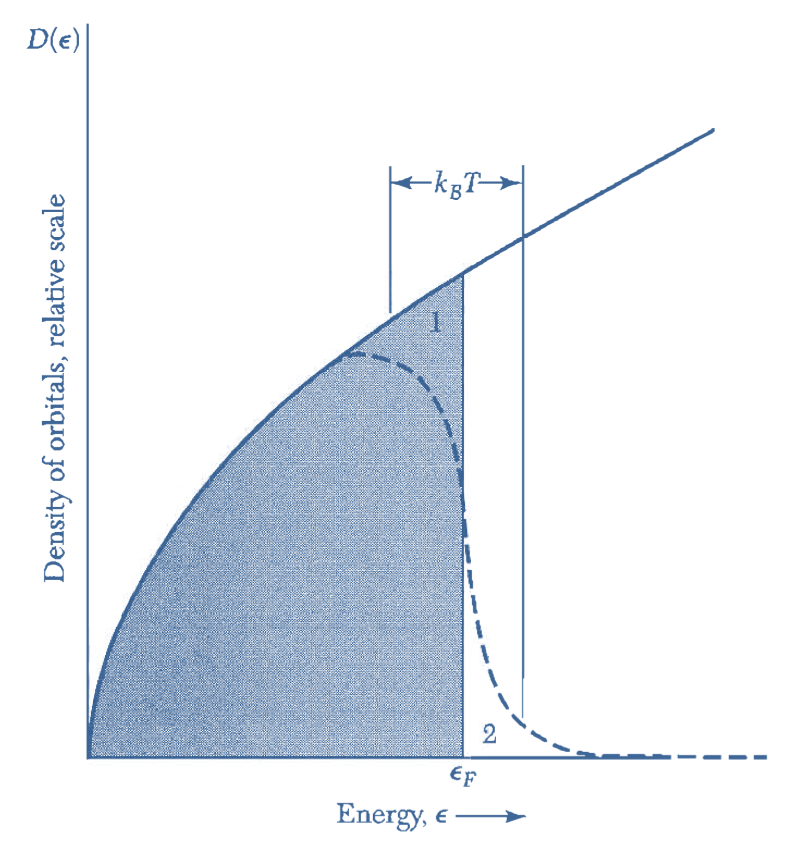
\includegraphics[width=0.8\textwidth]{figures/usomm.png}
  \caption{Al reducir la temperatura, el escalón (de anchura
    aproximada $\kb  T$) se vuelve más
    acusado. Para ello, electrones pasan de la región 2 a la región 1.}
  \label{fig:usomm}
\end{figure}
Por lo tanto el calor específico es
\begin{equation}
  c_v = \pfrac{U}{T} = \frac{2N\kb ^2 T}{\varepsilon_F} \propto T
\end{equation}
Recordar que en los fonones $c_v \propto T^2$.

El calor específico clásico es $\frac{3}{2}N\kb $, la corrección echa
es de un factor 100 a temperatura ambiente y con parámetros
típicos. Es también el factor de error en $c_v$ que poseía el modelo
de Drude.

\subsection{Cálculo preciso}
\label{subsec:accurate}

Utilizamos la expansión de Sommerfield (eq. \ref{eq:somm} ):
\begin{equation}
  U(T) = U(0) + \frac{\pi^2}{6}(\kb  T)^2 D(\varepsilon_F)
\end{equation}
Derivando, obtenemos el calor específico. Recordar que
$D(\varepsilon_F) = \frac{3N}{2\varepsilon_F}$:
\begin{equation}
  c_v = \frac{\pi^2 \kb ^2 T N}{2 \varepsilon_F} = \gamma T
\end{equation}
donde a $\gamma$ se le denomina \emph{parámetro de Sommerfield}. No
obstante, esto no es el calor específico del metal ya que falta
sumar la contribución de los fonones ,mucho mayor excepto a baja
temperatura, como puede verse en la figura
\ref{fig:electronvsphononcv}. Si la temperatura es muy
inferior a la de Fermi y a la de Debye ($T_F \sim 10^4 \ \text{K}$,
pero $\Theta_D \sim 300 \ \text{K}$) tenemos
\begin{equation}
  c_v = c_{v,e^{-}} + c_{v,\text{ph}} = \gamma T + \beta T^3
\end{equation}
$\gamma$ no encaja bien con los resultados experimentales
(en los peores casos - los llamados \emph{heavy fermions}- difiere en
un factor $10^3$). La solución pasa por contemplar la interacción de
los electrones con el potencial periódico de la red y la consecuente
teoría de bandas. Esta me da una masa efectiva que cambia el valor de
$\varepsilon_F$ y me corrige $\gamma$; dicha masa efectiva puede ser
mayor o menor que la del electrón.

Las interacciones electrón-electrón, al igual que las interacciones
electrón-fonón, también aumentan la masa efectiva.

El principal fallo de este modelo está en suponer que de
$D(\varepsilon) \propto \sqrt \varepsilon$. Esta aproximación para $D(\varepsilon)$ funciona bien con
electrones del tipo \emph{s}, pero falla estrepitosamente para
electrones de otros tipos (\emph{p,d,f}...) como puede verse en la
figura \ref{fig:spdf}. La plata, por ejemplo,
con un electrón \emph{s} en la banda de conducción, tiene un buen
ajuste para $\gamma$.

\begin{figure}
  \centering
  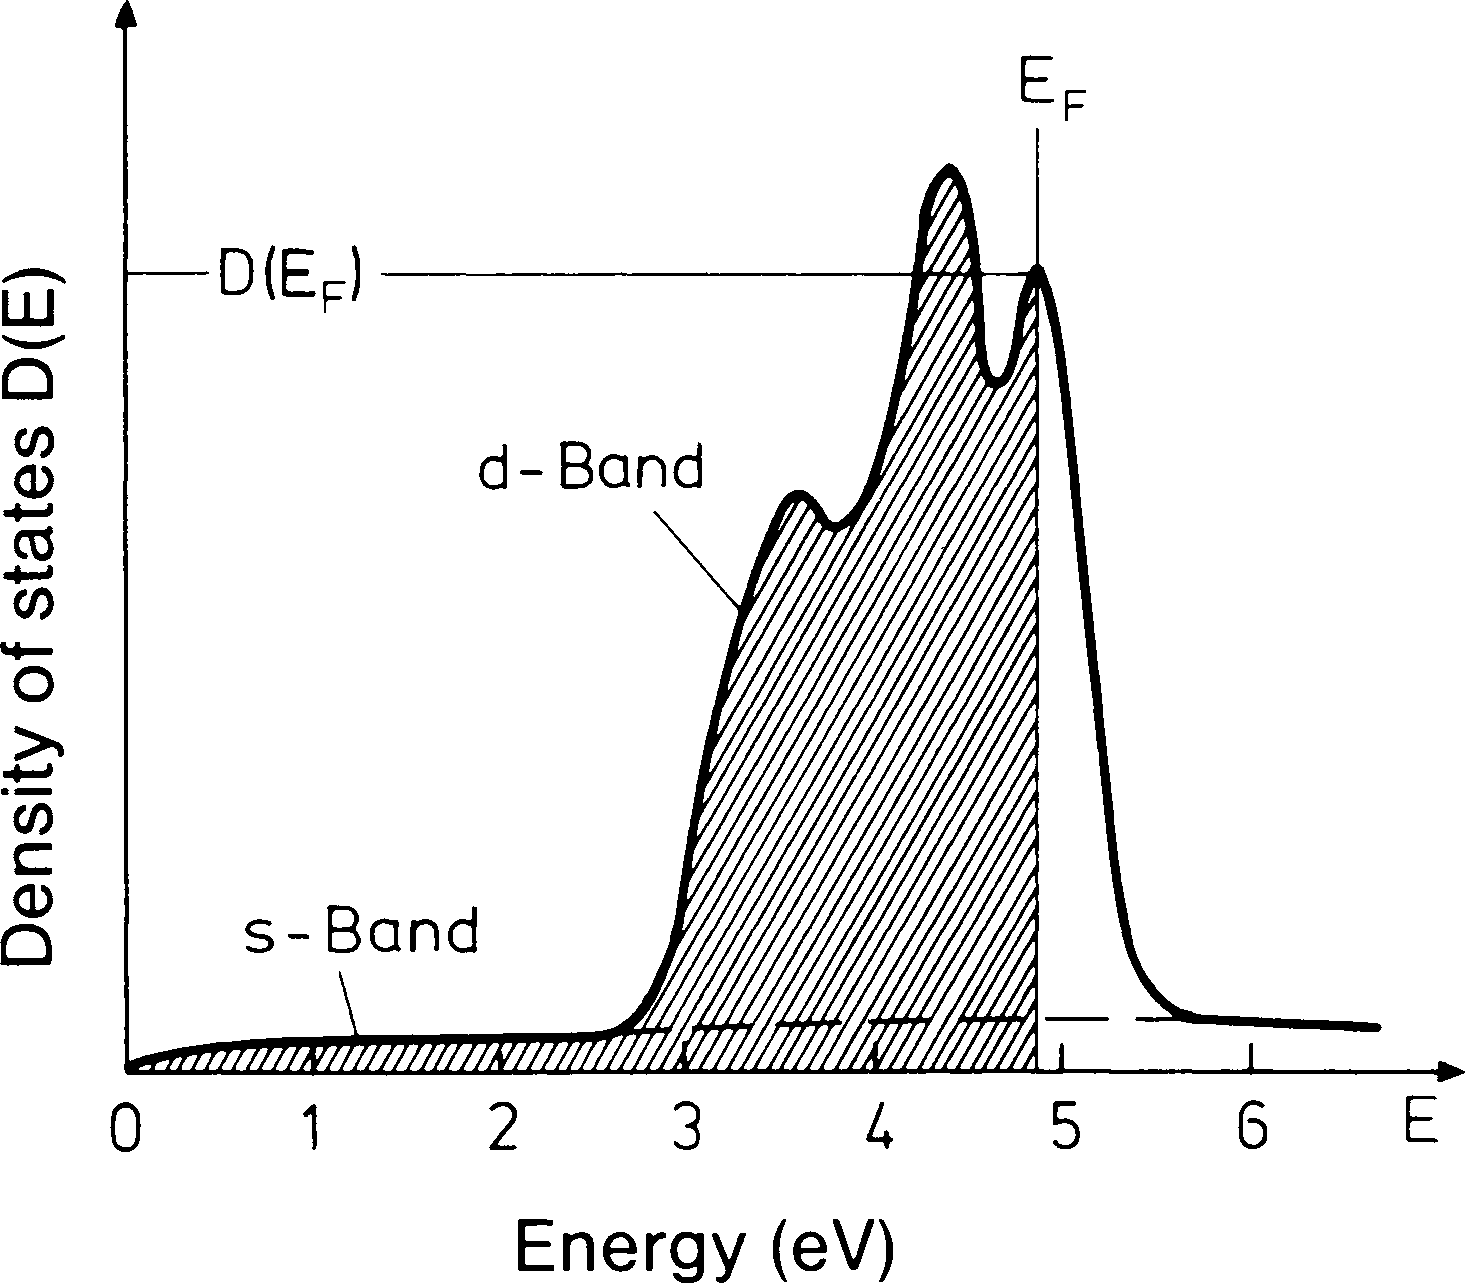
\includegraphics[width=0.8\textwidth]{figures/spdf.png}
  \caption{Los electrones \emph{s} tienen una forma funcional muy
    similar a $\sqrt x$, no así los del tipo \emph{d}. Estos últimos
    tienen una contribución en la densidad de estados de incluso un orden
  de magnitud, por lo que ignorarlos puede introducir grandes errores
  en los modelos.}
  \label{fig:spdf}
\end{figure}

\section{Propiedades del gas de Fermi}
\label{sec:fermiprop}
Partimos de que el trabajo de un electrón en un campo externo $E$ es
\begin{equation}
  \delta E = -e E v_g \cdot \delta t
\end{equation}
Hallamos la relación entre $\delta E$ y $\delta k$:
\begin{equation}
  \delta E = \frac{\text{d}E}{\text{d}k}\delta k =
  \frac{\text{d}\hbar\omega}{\text{d}k} \delta k = \hbar
  \frac{\text{d}\omega}{\text{d}k}\delta k = \hbar v_g \delta k
\end{equation}
Por tanto hallamos que $\delta E = \hbar v_g \delta k = -e E v_g
\delta t$ y en 3D:
\begin{equation}
  \hbar \frac{\text{d}\mathbf{k}}{\text{d}t} = -e \mathbf{E} = \mathbf{F}
\end{equation}
En una dimensión podemos escribir
\begin{equation}
  \text{d} k_x = \frac{-e E_x}{\hbar} \text{d}t \ \rightarrow \ \delta
  k_x  \sim \delta k_x \tau
\end{equation}
La esfera de Fermi se desplaza a la derecha una cantidad $\delta k_x$
muy pequeña; los procesos de relajación la devolverán al
equilibrio. Esto marca una diferencia fundamental con el modelo de
Drude: no todos los electrones contribuyen a la corriente, sino solo
unos pocos. Como se verá, en lugar de desplazarse a una pequeña
velocidad todos por igual (modelo de Drude) se desplazan todos los que
están fuera de equilibrio a velocidad $v_F$.

Como los componentes del gas de electrones son fermiones los procesos
de scattering no pueden llevar electrones a estados ocupados, lo que
implica que han de atravesar toda la esfera de Fermi para volver al equilibrio
(fig. \ref{fig:fermiscattering}). Los procesos de scattering han de ser capaces
de cambiar mucho la $\mathbf{k}$ del electrón (la esfera de Fermi es
de aproximadamente el tamaño de la primera zona de Brillouin), han de
ser interacciones o con impurezas o con fonones de alta
$\mathbf{q}$. Expresando esto en función de $\tau$ obtenemos la
\emph{regla de Matthiessen}:
\begin{equation}
  \frac{1}{\tau} = \frac{1}{\tau_i} + \frac{1}{\tau_L (T)}
\end{equation}
donde $\tau_i$ es el término debido a las colisiones con impurezas y
$\tau_L(T)$ el debido a la interacción electrón-fonón, que depende de
la temperatura por depender el número de fonones de $T$ (es nulo a
temperatura nula por no quedar fonones). Esta regla
implica que la resistividad, que es proporcional a $\tau^{-1}$
($\rho = \sigma^{-1} = \left( \frac{ne^2 \tau}{m} \right)^{-1} \propto
\tau^{-1}$) converge en temperatura nula a un valor constante dado por
las impurezas del sólido:
\begin{equation}
\begin{split}
  \lim_{T\to 0} \rho &= \lim_{T\to 0} \frac{m}{ne^2} \frac{1}{\tau} =
  \\ &=
  \lim_{T\to 0} \frac{m}{ne^2} \frac{1}{ \tau_i + \cancel{\tau_L(T)}}= \\ &= \frac{m}{ne^2}
                                          \frac{1}{\tau_i} \propto
                                          \tau_i ^{-1}
\end{split}
\end{equation}

\begin{figure}
  \centering
  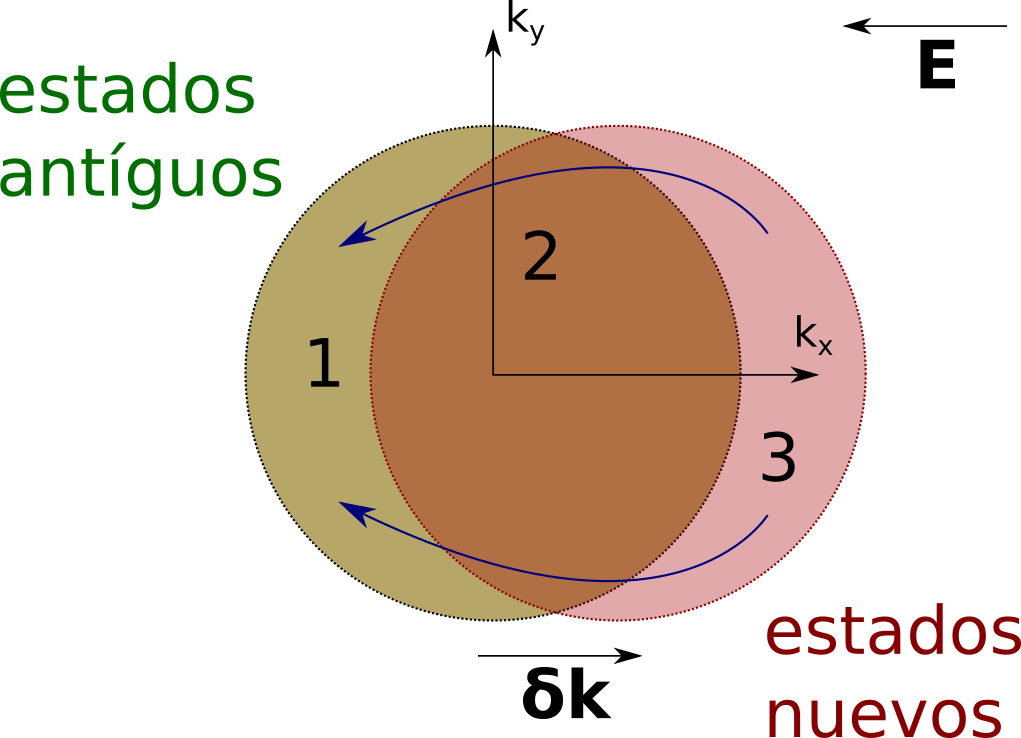
\includegraphics[width=0.8\textwidth]{figures/fermiscattering.png}
  \caption{Los electrones pasan de la esfera vieja (zonas 1 y 2) a la
    nueva (zonas 2 y 3). Los procesos de relajación llevan a los
    electrones fuera del equilibrio (zona 3, la única no presente en
    la esfera de Fermi original) a la esfera vieja. Estos podrían ir a
  la zona 2, pero esta ya está ocupada por electrones, así que sólo
  les queda ir a la zona 1, atravesando toda la esfera.}
  \label{fig:fermiscattering}
\end{figure}

\subsection{Conductividad eléctrica}

Tenemos que
\begin{equation}
  \rho (T) = \frac{m}{n e^2 \tau(T)}
\end{equation}
Veamos la influencia de los procesos N, ya que son mayoritarios y
contribuyen a $\rho$ en metales (no así a la conductividad térmica).

\subsubsection{Altas temperaturas}
Si las temperaturas son mucho más altas que la de Debye,
\begin{equation}
  \langle n_q \rangle \sim \frac{1}{\left[ 1 + \frac{\hbar
        \omega(q)}{\kb  T} \right] - 1} = \frac{\kb  T}{\hbar\omega(q)}
\end{equation}
Como $\tau ^{-1} \propto \langle n_q\rangle \propto T$ (el principal
mecanismo que limita el recorrido libre medio son las colisiones
electrón-fonón), tenemos que $\rho \propto T$.

% El momento de los fonones es más o menos del orden de $\hbar q_D$
% con $q_D$ del orden de $\frac{1}{a}$ ya que
% subir la temperatura no aumenta la energía de los fonones (ya es
% máxima), sino su número.
% \begin{equation}
%   \hbar \omega(q) \sim \hbar \omega_D \rightarrow q \sim q_D \sim \frac{1}{a}
% \end{equation}
% La $\mathbf{k}$ de los electrones ha de cambiar completamente de
% sentido y cruzar la esfera de Fermi.


\subsubsection{Bajas temperaturas}
\label{subsubsec:lowtempelectron}
A temperaturas mucho menores que las de Debye el scattering de
electrones por fonones sigue siendo el mecanismo que genera la mayor parte de la
resistividad. la energía de los fonones esta dominada por la agitación térmica, $\hbar \omega(q) <
\kb T$.

Deducimos que, debido al principio de exclusión de Pauli, los electrones interactuantes han
de tener una energía similar a $\kb  T$ para poder pasar a una zona
desocupada; en la figura \ref{fig:usomm} vemos como la única zona en la que hay
posibles transiciones es la cercana a la energía por agitación
térmica, especialmente a bajas temperaturas, cuando el escalón se
vuelve más acusado.

Dichos electrones tienen una $q$ muy pequeña, por lo que los procesos de
scattering tienen un ángulo prácticamente nulo
(fig. \ref{fig:smalltheta}). Por tanto, necesito procesos a varios
fonones para que los electrones vuelvan al equilibrio:
\begin{equation}
  \frac{1}{\tau_L} \propto \langle n_q \rangle (1-\cos \theta)
\end{equation}
donde el término angular da cuenta de la efectividad de la colisión;
los fonones en dirección contraria a los electrones son más efectivos
para ``girarlos''.

La dependencia térmica del proceso está implícita en el ángulo (ver
geometría en la figura \ref{fig:smalltheta}):
\begin{equation}
  \sin \frac{\theta}{2} = \frac{q/2}{k_F} \sim \frac{\theta}{2}
\end{equation}
Por tanto,
\begin{equation}
  1 - \cos \theta \sim \left( \frac{\theta}{2} \right)^2 \sim \left(
    \frac{q}{2k_F} \right) ^2 \propto q^2 = \left(
    \frac{\omega(q)}{v_s} \right)^2 \sim \left( \frac{\kb  T}{v_s}
  \right) ^2 \propto T^2
\end{equation}
Teniendo en cuenta que la densidad de estados de los fonones va como $T^3$ (modelo de
Debye), la resistividad por interacción electrón-fonón queda como
\begin{equation}
\label{eq:t5}
  \rho_L \propto \frac{1}{\tau_L} = \langle n_q \rangle (1 - \cos
  \theta) \propto T^3 T^2 = T^5
\end{equation}

Notar como la resistividad se desvía de la ley $T^3$ por la influencia
de los ángulos de scattering; a esto se le denota \emph{ley de Bloch
  de la resistividad}.

\begin{figure}
  \centering
  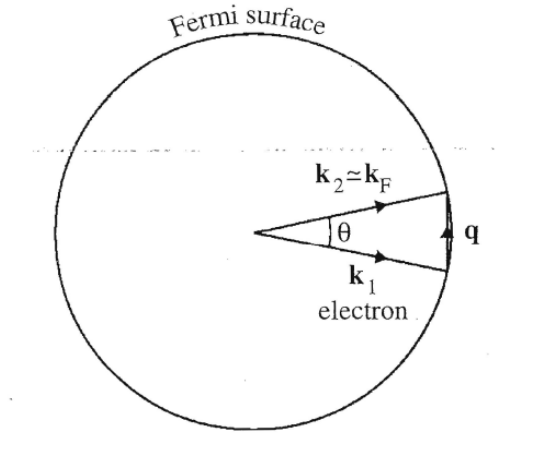
\includegraphics[width=0.5\textwidth]{figures/smalltheta.png}
  \caption{Scattering de un electrón de vector de ondas $\mathbf{k}$
    por un fonón con vector de ondas $\mathbf{q}$. Los procesos de scattering electrón-fonón a baja
    temperatura tienen bajo ángulo por el pequeño módulo de los
    fonones implicados.}
  \label{fig:smalltheta}
\end{figure}


Los procesos U añaden desviaciones adicionales a la ley $T^5$ recién
hallada.

\paragraph{Procesos U}
Los procesos que no pueden existir como procesos N (por las
limitaciones de la primera zona de Brillouin) pueden existir como
procesos Umklapp (figura \ref{fig:uprocess}).

\begin{figure}
  \centering
  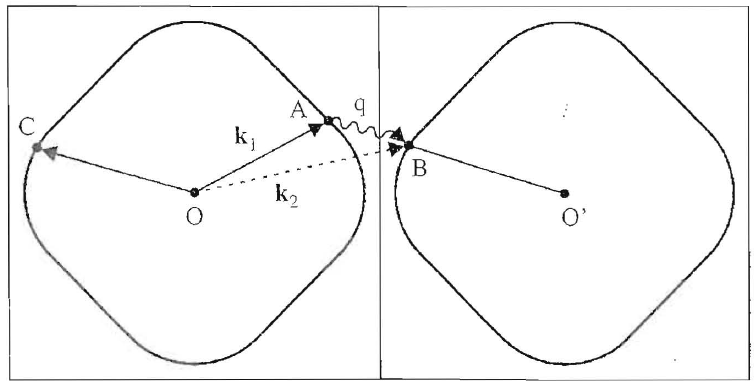
\includegraphics[width=0.8\textwidth]{figures/uprocess.png}
  \caption{Para pasar de A a C los electrones pueden emplear fonones
    de baja $\mathbf{q}$ y volver a la PZB si se ayudan de un vector $\mathbf{G}$ de la
    red recíproca.}
  \label{fig:uprocess}
\end{figure}

La geometría de la esfera de Fermi respecto a la PZB es influyente (la
esfera de Fermi no tiene por qué tener forma esférica si no son electrones
libres). Estos ``encajes'' de la esfera de Fermi con la red recíproca
determinan si hay o no procesos U (fig. \ref{fig:encaje}), dándonos un
vector de ondas mínimo para los fonones, que determina un
$\omega_\text{min}$. Como $\kb  T l \hbar \omega_\text{min}$, el
número de fonones es $n(q_\text{min}) \sim
\exp(-\frac{\hbar\omega_\text{min}}{\kb  T}) =
e^{\frac{-\theta_F}{T}}$ con $\theta_F$ un factor dependiente de la
geometría. La colaboración a la resistividad por estos procesos queda como
\begin{equation}
  \rho_\text{U} \propto \frac{1}{\tau} \propto \langle n_q \rangle \propto
  e^{\frac{-\theta_F}{T}}
\end{equation}

\begin{figure}
  \centering
  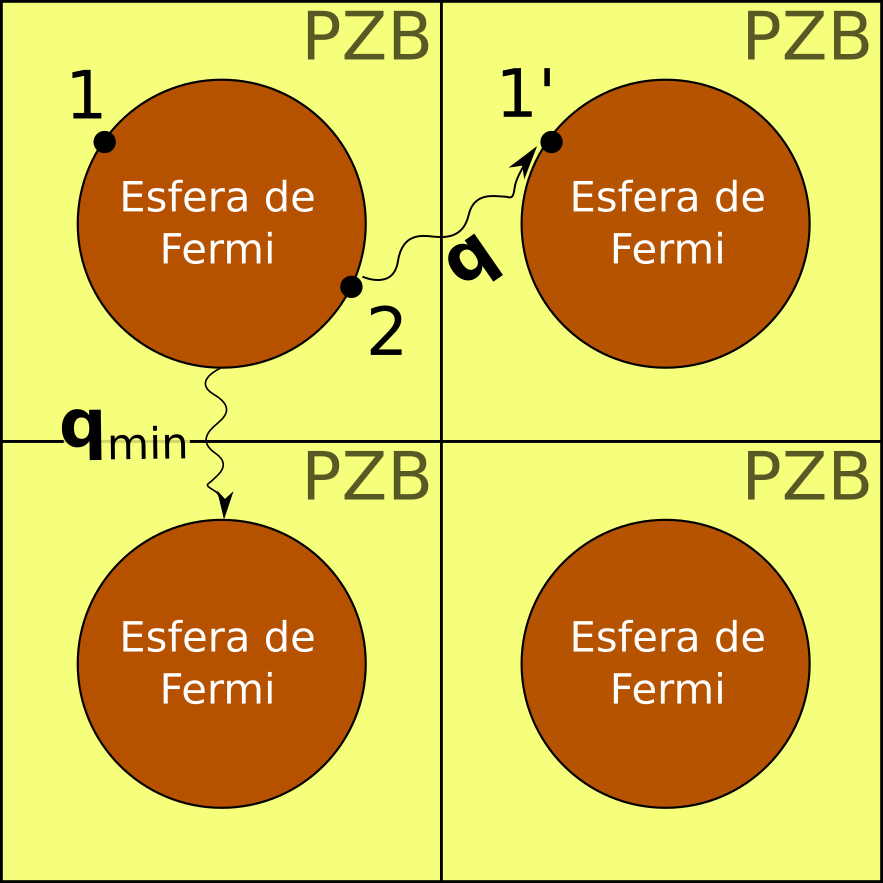
\includegraphics[width=0.8\textwidth]{figures/encaje.png}
  \caption{Para pasar de 2 a 1 el electrón puede ayudarse de un
    proceso U que le transporte  a 1' mediante un fonón $\mathbf{q}$ y le
    devuelva a 1 con un $\mathbf{G}$. Este proceso nos da una
    $\mathbf{q}_\text{min}$, en este caso la separación entre las esferas.}
  \label{fig:encaje}
\end{figure}

\subsubsection{Temperaturas prácticamente nulas}
A ultrabaja temperatura el único scattering de los electrones es
debido a las impurezas. Obtenemos por tanto que $\rho \to \text{cte.}$




\subsection{Conductividad térmica}
Los elementos que más aportan a la conductividad térmica de un metal
son sus electrones. En aleaciones con estructura poco ordenada o
muestras con muchas impurezas la conductividad térmica otorgada por la
red puede llegar a ser comparable a la electrónica.

Veamos la contribución electrónica.
Sabemos que $\kappa = \frac{1}{3} v^2 \tau c_v$, con $v \sim
v_{\scriptscriptstyle F}$ ya que sólo participan
los electrones del exterior de la esfera de Fermi. Con
$c_v = \gamma T = \frac{\pi^2 n \kb ^2}{2 \epsilon_{\scriptscriptstyle
  F}} T$:
\begin{equation}
  \kappa = \cdots = \frac{1}{3} \frac{\pi^2 n \kb ^2}{m} T
\end{equation}
donde se ha utilizado que $\varepsilon_{\scriptscriptstyle F} =
\frac{1}{2}m v_{\scriptscriptstyle F}^2$.

El coeficiente de la ley de Wiedemann-Franz, con $\sigma = \frac{n e^{2} \tau}{m}$,
queda como
\begin{equation}
  L = \frac{\kappa}{\sigma T} = \cdots = \frac{\pi^3}{3} \left(
    \frac{\kb }{e} \right)^2 \sim 2.45 \cdot 10^{-8} \si{\watt\ohm\per\kelvin}
\end{equation}
El valor coincide muy bien con el experimental, no como el de Drude
que sufría de un factor 2 de error.
\begin{equation}
  \frac{L}{L_\text{Drude}} = \frac{2\pi^2}{9} \sim 2.19
\end{equation}

En el efecto Seebeck la discrepancia es mayor:
\begin{equation}
  \begin{cases}
    Q &= \frac{-1}{3ne} c_v = \frac{-1}{6ne} \frac{\pi^2 n
      \kb ^2}{\varepsilon_F} T\\
    Q_\text{Drude} &= \frac{-1}{3ne} c_v = \frac{-\kb }{2e}
  \end{cases} \ \ \ \rightarrow \ \ \frac{Q}{Q_\text{Drude}} =
  \frac{1}{100} \text{@} \SI{100}{\kelvin}
\end{equation}

\subsubsection{Dependencia térmica de $\kappa$}
Suponemos temperaturas suficiente bajas como para asumir $TlT_F$
(buena aproximación, pues a la temperatura de Fermi casi todos los
metales ya están fundidos y no hay sólido con el que
trabajar). Tenemos entonces que $c_v \sim \gamma T$ y por tanto
\begin{equation}
  \kappa(T) = \frac{1}{3} v_\text{ph}^2  \tau(T)c_v(T) \propto T \tau(T)
\end{equation}
Si la temperatura es mucho mayor que la de Debye,
\begin{equation}
  \frac{1}{\tau} \propto T \ \rightarrow \ \kappa(T \gg \theta_D) \propto T\cdot
  \frac{1}{T} = \text{cte.}
\end{equation}

Si la temperatura es mucho menor que la de Debye,
\begin{equation}
  \label{eq:t3}
  \underbrace{\frac{1}{\tau}\propto T^3}_{\text{Debye model}} \ \rightarrow
  \ \kappa(T) \propto T \cdot \frac{1}{T^3} = T^{-2}
\end{equation}
Y si la temperatura es prácticamente nula,
\begin{equation}
  T \sim 0 \ \rightarrow \  \frac{1}{\tau} \sim \text{cte.} =
  \frac{1}{\tau_i} \ \rightarrow \ \kappa(T) = T\cdot \text{cte.}
\end{equation}
Pueden verse más detalles en el apéndice \ref{app:thermaldep}
\subsubsection{Ley de Wiedemann-Franz en zona intermedia}
Notar como estos resultados implican que la ley de Wiedemann-Franz no
se cumple en la zona intermedia, ya que las $\tau$ de numerador y
denominador no son cancelables. En el numerador tenemos la $\tau$ por
$\kappa$ que es proporcional a $T^{-3}$ (eq. \ref{eq:t3})y en el denominador la $\tau$
por $\sigma$ que es proporcional a $T^{-5}$ (eq. \ref{eq:t5}).

\chapter{Electrones en potencial periódico}
Los modelos vistos hasta ahora tienen algunas deficiencias:
\begin{itemize}
\item No hay ninguna distinción entre metales, semimetales y
  aislantes.
\item En los efectos de Hall y de Seebeck los coeficientes son
  estrictamente positivos.
\item No hay ninguna relación entre los electrones de conducción y los
  de valencia.
\item No hay efectos de magnetotransporte.
\end{itemize}
Estas deficiencias\footnote{El capítulo 3 del Ashcroft comenta más
  fallos de los modelos con más detalle.} vienen de la consideración
de electrones libres, sin contemplar las interacciones
electrón-electrón ni las interacciones electrón-red. Además, estamos
limitados por la aproximación de tiempo de relajación.

Por último, los modelos considerados asumen que se aportan todos los
electrones de valencia a la conducción, lo cual es falso.

\section{Teorema de Bloch}
Veamos qué pasa con la interacción de los electrones con la red.

El potencial ha de ser, debido a la periodicidad de la red,
\begin{equation}
  U(\mathbf{r}) \ \ | \ \  U(\mathbf{r}) = U(\mathbf{r}+\mathbf{R})
\end{equation}
quedando la ecuación de Schrodinger como
\begin{equation}
  \left[ \frac{-\hbar}{2m} \nabla ^2 + U(\mathbf{r}) \right] \psi = E \psi
\end{equation}
El \emph{teorema de Bloch} (en una dimensión se llama \emph{teorema de
Floquet}) me dice que
\begin{equation}
  \boxed{
  \psi_\mathbf{k}(\mathbf{r}) = e^{i \mathbf{k} \mathbf{r}}
  u_\mathbf{k}(\mathbf{r})  }
\end{equation}
es decir, la función de ondas $\psi_\mathbf{k}$ es una onda plana
modulada por una función periódica de la red. De manera alternativa,
el teorema puede expresarse como
\begin{equation}
  \begin{split}
    \psi(\mathbf{r}+\mathbf{R}) = e^{i \mathbf{k}\mathbf{r}}e^{i
      \mathbf{k}\mathbf{R}} u(\mathbf{r}+\mathbf{R}) &=    e^{i \mathbf{k}\mathbf{r}}e^{i
      \mathbf{k}\mathbf{R}} u(\mathbf{r}) = e^{i \mathbf{k}\mathbf{R}}
    \psi(\mathbf{r}) \\
   \psi(\mathbf{r}+\mathbf{R}) &= e^{i \mathbf{k} \mathbf{R}}
  \psi(\mathbf{r})
  \end{split}
\end{equation}
Ambas formulaciones del teorema de Bloch son completamente equivalentes.
\begin{boldproof}[Demostración del teorema de Bloch]
 Comenzamos por introducir el operador ``traslación por un vector de
 la red'', $T_\mathbf{R}$, definido como
\begin{equation}
  T_\mathbf{R} f(\mathbf{r}) = f(\mathbf{r}+\mathbf{R})
\end{equation}
El operador conmuta con $\mathcal{H}$:
\begin{equation}
  T_\mathbf{R}[ \mathcal{H}\psi ] = \mathcal{H}(\mathbf{r} + \mathbf{R})
  \psi(\mathbf{r}+\mathbf{R}) = \mathcal{H}(\mathbf{r})
  [T_\mathbf{R}\psi(\mathbf{r})] = \mathcal{H} [T_\mathbf{R}\psi], \ \ \forall \psi
\end{equation}
Donde se ha usado que la energía de la red $U(\mathbf{r})$ ha de ser
invariante ante traslación para escribir $\mathcal{H}(\mathbf{r}) = \mathcal{H}(\mathbf{r}+\mathbf{R})$.

Al conmutar, podemos escoger una base de autovalores común a ambos
operadores:
\begin{equation}
  \begin{cases}
    \mathcal{H} \psi &= E \psi \\
    T_\mathbf{R} \psi &= c(\mathbf{R}) \psi
  \end{cases}
\end{equation}
Además,
\begin{equation}
  T_\mathbf{R}T_\mathbf{R'} \psi =
  T_\mathbf{R}\psi(\mathbf{r}+\mathbf{R'}) =
  \psi(\mathbf{r}+\mathbf{R'}+\mathbf{R}) = T_{\mathbf{R+R'}}\psi
\end{equation}
De esta última propiedad deduzco que $c(\mathbf{R})c(\mathbf{R'}) =
c(\mathbf{R}+\mathbf{R'})$. La normalización de la función de ondas
nos indica que
\begin{equation}
  \int |\psi(\mathbf{r}+\mathbf{R})|^2 \ \text{d}\mathbf{r} = |
  c(\mathbf{R}) |^2 \int |\psi(\mathbf{r})|^2 \ \text{d}\mathbf{r}
\end{equation}
Donde se ha usado que $|\psi(\mathbf{r}+\mathbf{R})| = | T_\mathbf{R}
\psi(\mathbf{r})| = | c(\mathbf{R}) \psi(\mathbf{r})| = |
c(\mathbf{R}) ||\psi(\mathbf{r})|$. Por tanto, $|c(\mathbf{R})| = 1$ y
$c(\mathbf{R}) = e^{i \theta (\mathbf{R})}$. Utilizando que $c(\mathbf{R})c(\mathbf{R'}) =
c(\mathbf{R}+\mathbf{R'})$, obtenemos que una posible función
candidata a $\theta$ es $\mathbf{k}\mathbf{R}$. Se tiene entonces que
\begin{equation}
  c(\mathbf{R}) = e^{i \mathbf{k}\mathbf{R}}
\end{equation}
y por tanto
\begin{equation}
  T_\mathbf{R} \psi(\mathbf{r}) = \underbrace{c(\mathbf{R})}_{e^{i
      \mathbf{k} \mathbf{R}}}\psi(\mathbf{r}) = \psi(\mathbf{r}+\mathbf{R})
\end{equation}
Obteniéndose que $\psi(\mathbf{r}+\mathbf{R}) = e^{i
  \mathbf{k}\mathbf{R}} \psi (\mathbf{r})$.
\end{boldproof}

\subsubsection*{Condiciones de contorno}
Utilizo condiciones de contorno periódicas, de forma que, por
ejemplo,
\begin{equation}
  \psi_\mathbf{k}(x+L_x, y,z) = \psi_\mathbf{k}(x,y,z) \ \rightarrow \
  e^{i k_x (x+L_x)} = e^{i k_x x}
\end{equation}
Obtenemos tras aplicar esto a las 3 coordenadas espaciales que
\begin{equation}
  \psi(\mathbf{r} + N_i \mathbf{a}_i) = \psi(\mathbf{r}), \ \
  \begin{cases}
    &i \in \{ 1,2,3\} \\
    &N_1N_2N_3 = N
  \end{cases}
\end{equation}
Aplicando el teorema de Bloch obtengo a estas condiciones de contorno obtengo
\begin{equation}
  \psi(\mathbf{r}+N_i \mathbf{a}_i) = e^{i \mathbf{k} N_i
    \mathbf{a}_i} \psi(\mathbf{r}) = \psi(\mathbf{r})
\end{equation}
y por tanto $i \mathbf{k}N_i \mathbf{a}_i = 2\pi n_i i, \ \ n_i\in
\mathbb{Z}$. Como $ \mathbf{k} = \sum_{i=\{1,2,3\}} k_i \mathbf{b}_i$
y $\mathbf{a}_i \mathbf{b}_j = 2\pi\delta_i^j$, tengo que $N_i k_i
2\pi = 2\pi n_i$ y $k_i= \frac{n_i}{N_i}, \ \ i\in\{1,2,3\}$.

La densidad de estados en $\mathbf{k}$ será
\begin{equation}
  D(\mathbf{k}) = \frac{V}{(2\pi)^3} \cdot 2 = \frac{V}{4\pi^3}
\end{equation}

\section{Consecuencias del teorema de Bloch}
\begin{enumerate}
\item $\hbar \mathbf{k}$ ya no es el momento del electrón.

El operador momento en mecánica cuántica es $-i \hbar
\nabla$. Aplicándoselo a una función de ondas de un electrón Bloch
obtengo
\begin{equation}
\begin{split}
  -i \hbar \psi_\mathbf{k}(\mathbf{r}) &= -i \hbar \nabla
\left[ e^{i \mathbf{k} \mathbf{r}} {u} (\mathbf{r}) \right] = \\ &= -i
\hbar i \mathbf{k} e^{i \mathbf{k} \mathbf{r}} {u}(\mathbf{r}) - i
\hbar e^{i \mathbf{k}\mathbf{r}} \nabla {u}(\mathbf{r}) = \\ &= \hbar
\mathbf{k} \psi_\mathbf{k}(\mathbf{r}) - \underbrace{i \hbar e^{i
\mathbf{k}\mathbf{r}} \nabla {u}_\mathbf{k}(\mathbf{r})}_{\text{extra
term}}
\end{split}
\end{equation}
al término $\hbar \mathbf{k}$ se le denota, al igual que con los
fonones, \emph{cuasimomento}. Notar que el momento ya no es paralelo a
$\mathbf{k}$, como ocurría con los electrones libres.
\item Siempre puede tomarse un $\mathbf{k}\in \text{PZB}$.

Si un $\mathbf{k'}$ ne está en la primera zona de Brillouin, lo
escribimos como $\mathbf{k'} = \mathbf{k}\in \text{PZB} +
\mathbf{G}$, y tenemos que
\begin{equation}
\begin{split}
  \psi(\mathbf{r}+\mathbf{R}) &= e^{i \mathbf{k'} \mathbf{R}}
  \psi(\mathbf{r}) = e^{i(\mathbf{k}+\mathbf{G})}\psi(\mathbf{r}) =
  \\ &=
  e^{i \mathbf{k} \mathbf{R}} \cancelto{1}{e^{i \mathbf{G}
      \mathbf{R}}} \psi(\mathbf{r}) = e^{i \mathbf{k} \mathbf{R}} \psi(\mathbf{r})
\end{split}
\end{equation}
\item Necesitamos un índice adicional $n$.

Si no, existe ambiguedad en
${u}_\mathbf{k}(\mathbf{r})$. Tratemos de resolver la ecuación
de Schrodinger, $\mathcal{H} \psi = \varepsilon \psi$:
\begin{equation}
  \begin{split}
    \mathcal{H} \psi_\mathbf{k}(\mathbf{r}) &= \varepsilon
    \psi_\mathbf{k}(\mathbf{r}) \\
\left[ \frac{- \hbar^2}{2m} \nabla
      ^2 + U(\mathbf{r}) \right] \left[ e^{i \mathbf{k} \mathbf{r}}
      u_\mathbf{k}(\mathbf{r}) \right]   &=  \varepsilon_\mathbf{k}
    e^{i \mathbf{k} \mathbf{r}} u_\mathbf{k}(\mathbf{r})
  \end{split}
\end{equation}
En el término del laplaciano, tenemos
\begin{equation}
  \begin{split}
-\nabla^2 \left[ e^{i \mathbf{k}\mathbf{r}}  u_\mathbf{k}(\mathbf{r})
\right] &= -\nabla \left[ i \mathbf{k} e^{i \mathbf{k}\mathbf{r}}
  u_\mathbf{k} +  e^{i \mathbf{k}\mathbf{r}} \nabla ^2 u_\mathbf{k}
\right] \\
 &= \mathbf{k}^2 e^{i \mathbf{k} \mathbf{r}} u_\mathbf{k} - 2 i
\mathbf{k} e^{i \mathbf{k} \mathbf{r}} \nabla u_\mathbf{k} - e^{i
  \mathbf{k} \mathbf{r}} \nabla ^2 u_\mathbf{k} = \\
&= (\mathbf{k}-i\nabla)^2 e^{i \mathbf{k} \mathbf{r}} u_\mathbf{k}
  \end{split}
\end{equation}
Obteniendo
\begin{equation}
  \begin{cases}
  \left[ \frac{\hbar^2}{2m}(\mathbf{k} - i\nabla)^2 + U(\mathbf{r})
  \right] u_\mathbf{k} (\mathbf{r}) = \varepsilon_\mathbf{k}
  u_\mathbf{k}(\mathbf{r}) \\
  u_\mathbf{k} = u_\mathbf{k}(\mathbf{r}+\mathbf{R})
  \end{cases}
\end{equation}
que no es más que la ecuación de Schrodinger con condiciones de
contorno en un recinto cerrado (la primera zona de Brillouin). Al ser
un problema de autovalores en una región finita del espacio, tiene
infinitas soluciones, de manera análoga al pozo de potencial (problema
con infinitas soluciones discretas).

Por tanto, doy las funciones de onda como
\begin{equation}
  \psi_{n \mathbf{k}}(\mathbf{r}) = e^{i \mathbf{k} \mathbf{r}} u_{n\mathbf{k}}(\mathbf{r})
\end{equation}
donde el índice $n$, denotado \emph{índice de banda}, me indexa las
posibles soluciones.
\item Puedo elegir los índices de banda de forma que la periodicidad de
  las funciones sea justo la de la red.

\begin{equation}
  \exists n \ | \
  \begin{cases}
    \varepsilon_{n,\mathbf{k}} &=
    \varepsilon_{n,\mathbf{k}+\mathbf{G}} \\
    \psi_{n,\mathbf{k}} &= \psi_{n,\mathbf{k}+\mathbf{G}}
  \end{cases}
\end{equation}
A este conjunto de soluciones $\{\varepsilon_{n,\mathbf{k}} =
\varepsilon_n (\mathbf{k})\}$ se le denota \emph{estructura de bandas
  del sólido}. Al fijar la $n$, a los $\varepsilon_n (\mathbf{k})$ se
les denota \emph{bandas de energía}.
Como son funciones periódicas y contínuas\footnote{Notar que las
  $\mathbf{k}$ son contínuas porque el teorema de Bloch no les impone
  ninguna restricción. Posteriores imposiciones, como condiciones
  periódicas, pueden discretizar las $\mathbf{k}$.} en $\mathbf{k}$, han de
tener una cota superior e inferior (de manera análoga al $\sin x$).
\item En el tema de dinámica semiclásica veremos que puedo definir una
  velocidad electrónica promedio tal que
\begin{equation}
  \mathbf{v}_n(\mathbf{k}) = \frac{1}{\hbar} \nabla _\mathbf{k}
  \varepsilon_n (\mathbf{k})
\end{equation}
A $\mathbf{v}_n(\mathbf{k})$ se le llama \emph{velocidad promedio de la banda \emph{n}}.
\end{enumerate}

Notar que de momento sólo hemos levantado la restricción de no
interacción con la red. Los electrones siguen sin interaccionar entre ellos.

\section{Modelo 1D}
Vamos a resolver el modelo de Kronnig-Penney. Es un modelo 1D de
potencial periódico. Como potencial utilizamos (fig. \ref{fig:kronnigpot}):
\begin{equation}
  u(x) =
  \begin{cases}
    u_0, &x\in [a,b) \\
    0, & x\in (0,a)
  \end{cases}, \ \ u(x) = u(x+a+b)
\end{equation}


\begin{figure}
  \centering
    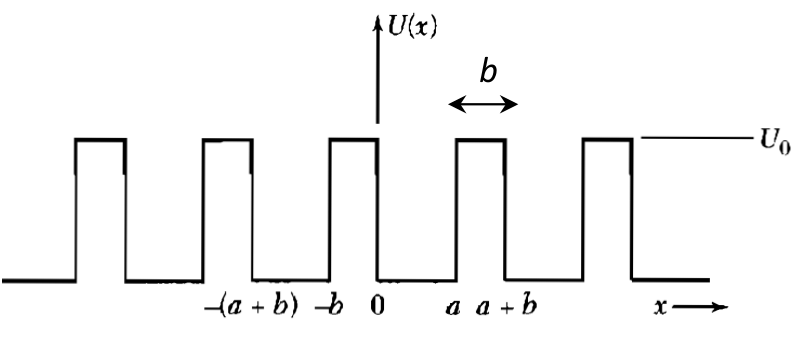
\includegraphics[width=0.6\textwidth]{figures/kronnigpot.png}
  \caption{Potencial periódico del modelo de Kronnig-Penney.}
  \label{fig:kronnigpot}
\end{figure}

Tras los correspondientes cálculos, obtenemos la ecuación para $\psi$:
\begin{equation}
  \psi = \
  \begin{cases}
    A e^{i\alpha x} + B e^{-i\alpha x} , &x\in(0,a) \\
    C e^{ \beta x} + D e^{- \beta x} , &x\in(-b,0) \\
  \end{cases}
\end{equation}
Donde $\alpha^2 = \frac{2m\varepsilon}{\hbar^2}$ y $\beta =
\frac{2m(\mu_0 - \varepsilon)}{\hbar^2}$.
Las demás zonas podemos calcularlas con el teorema de Bloch. Nuestro
parámetro de red es, en este caso, $a+b$. Por ejemplo:
\begin{equation}
  x\in(a,b) \ \rightarrow \ \psi_{x \in (a,b)} = e^{ik(a+b)}\psi_{x \in ({-b},0)}
\end{equation}
Tras una serie de cuentas\footnote{No pocas. La cosa es elegir
  $A,B,C,D$ tales que la función de ondas sea contínua en las
  transiciones entre pozos, lo que exige plantear dos sistemas de
  ecuaciones (continuidad en $x=0$ y $x=a$) y resolver un determinante
  (para obtener las soluciones no triviales). En palabras textuales
  del Kittel, ``\emph{Is rather tedious to obtain this equation}''.}, obtenemos
\begin{equation}
  \frac{\beta^2 -\alpha^2}{2 \beta \alpha } \sinh(\beta b) \sin(\alpha
  a) + \cosh(\beta b)\cos(\alpha a) = \cos[k(a+b)]
\end{equation}
Donde $\alpha^2 + \beta^2 = \frac{2m U_0}{\hbar^2}$. Utilizamos una
aproximación a deltas de Dirac para obtener una expresión más
analizable analíticamente:
\begin{equation}
  b\to0, \ U_0 \to \infty \ \ \ \rightarrow \ \ \ \frac{P}{\alpha a}
  \sin(\alpha a) + \cos (\alpha a) = \cos(ka)
\end{equation}
con $P = \frac{1}{2} \beta^2 b a$.

La ecuación tiene una solución numérica en forma de bandas de energía
(fig. \ref{fig:fullsolve}) predecible mediante métodos de análisis
gráfico (fig. \ref{fig:graphicsolve}.

\begin{figure}
  \centering
  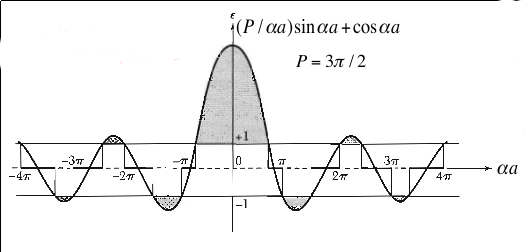
\includegraphics[width=0.8\textwidth]{figures/graphicsolve.png}
  \caption{Solución gráfica de
    $ \frac{P}{\alpha a} \sin \alpha a + \cos \alpha a = \cos ka$. Al
    ser $\cos ka$ una función acotada entre $\pm 1$, sólo existen
    soluciones para $\alpha$ en la zona sin sombrear. Las zonas
    sombreadas representan regiones energéticas para las que no existe
    una solución con forma de onda Bloch.}
  \label{fig:graphicsolve}
\end{figure}

\begin{figure}
  \centering
  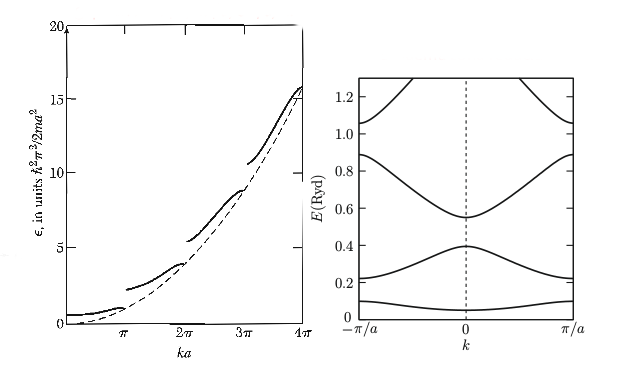
\includegraphics[width=0.8\textwidth]{figures/fullsolve.png}
  \caption{Energía en función de la longitud de onda para el modelo de
    Kronig-Penney en zona extendida y reducida. Se obtiene como la
    solución numérica de
    $ \frac{P}{\alpha a} \sin \alpha a + \cos \alpha a = \cos ka$.}
  \label{fig:fullsolve}
\end{figure}



\section{Ecuación central}
No es más que la ecuación de Schrodinger en un potencial periódico y
en momentos. Partamos por expresar el potencial periódico como una
suma de momentos:
\begin{equation}
  U(\mathbf{r}) = U(\mathbf{r}+\mathbf{R}) \stackrel{ \text{sec.}\
    \ref{sec:fper}}{\ \rightarrow \ } U(\mathbf{r}) =
  \sum_{\mathbf{G}} U_\mathbf{G} e^{i \mathbf{G}\mathbf{r}}
\end{equation}
donde los coeficientes vienen dados por:
\begin{equation}
  U_\mathbf{G} = \frac{1}{\boldsymbol{\Omega}} \int_\Omega
  \text{d}\mathbf{r}\ U(\mathbf{r}) e^{-i \mathbf{G} \mathbf{r}}
\end{equation}
como $U_\mathbf{G} \in \mathbb R$, tenemos que $U_\mathbf{G}^* =
U_\mathbf{-G}$ y ademas si $U_\mathbf{G}=U_\mathbf{-G}$ se tiene que
$U_\mathbf{G}^* = U_\mathbf{G}$.

Usualmente se toma $U_0 = \frac{1}{\Omega} \int_\Omega
\text{d}\mathbf{r} \ U(\mathbf{r}) = 0$ para tener el origen de
energías en el centro de la PZB (el llamado \emph{punto} $\Gamma$).

Tenemos una función de tipo Bloch; imponiendo condiciones de contorno
periódicas (o de Born-Von Karman):
\begin{equation}
  \psi(\mathbf{r}) = \sum_{\mathbf{q}} C_\mathbf{q} e^{i \mathbf{q}
    \mathbf{r}}, \ \
  \begin{cases}
    &\mathbf{q} = \sum_{\{1,2,3\}}\frac{m_i}{N_i} \mathbf{b}_i \\
    &m_i \in \mathbb Z
  \end{cases}
\end{equation}

Ya sólo resta sustituir todo en la ecuación de Schrodinger. El término
de la laplaciana queda como:
\begin{equation}
  \begin{split}
  -\nabla^2 \psi &= -\nabla^2 \left[ \sum_{\mathbf{q}} C_\mathbf{q}
    e^{i \mathbf{q} \mathbf{r}} \right] \\
  &= \sum_{\mathbf{q}} q^2 C_\mathbf{q} e^{i \mathbf{q} \mathbf{r}}
  \end{split}
\end{equation}
y el del potencial:
\begin{equation}
  \begin{split}
    u\psi &= \sum_{\mathbf{G}} U_\mathbf{G} e^{i \mathbf{G} \mathbf{r}}
    \sum_{\mathbf{q}} C_q e^{i \mathbf{q} \mathbf{r}} = \\ &=
    \sum_{\mathbf{G}, \mathbf{q}} U_\mathbf{G} C_\mathbf{q} e^{i(
      \mathbf{G} + \mathbf{q}) \mathbf{r}} \
    \stackrel{\mathbf{G}+\mathbf{q} = \mathbf{q'}}{=} \\
    &=\sum_{\mathbf{G}, \mathbf{q'}} U_\mathbf{G}
    C_{(\mathbf{q'}-\mathbf{G})} e^{i \mathbf{q'}\mathbf{r}} = \cdots
  \end{split}
\end{equation}

Como $\mathbf{q'}$ es un índice mudo puedo cambiarlo sin problemas por $q$.
\begin{equation}
  \cdots = \sum_{\mathbf{G}, \mathbf{q}} U_\mathbf{G}
  C_{(\mathbf{q}-\mathbf{G})} e^{i \mathbf{q} \mathbf{r}} = \cdots
\end{equation}

Puedo realizar la misma operación y cambiar $\mathbf{G}$ por
$\mathbf{G'}$:
\begin{equation}
  \cdots = \sum_{\mathbf{G'} , \mathbf{q}} U_\mathbf{G'}
  C_{(\mathbf{q}-\mathbf{G'})} e^{i \mathbf{q} \mathbf{r}}
\end{equation}
La ecuación de Schrodinger queda como
\begin{equation}
    \left( \frac{\hbar^2 q^2}{2m} - \varepsilon \right) C_\mathbf{q} +
    \sum_{\mathbf{G}} U_\mathbf{G'} C_{\mathbf{q}-\mathbf{G'}} = 0
\end{equation}
Por último, desplazo $\mathbf{q}$ de manera que la ecuación que en
función de $\mathbf{k}\in
\text{PZB}$, es decir, $\mathbf{q} = \mathbf{k} - \mathbf{G}$:
\begin{equation}
    \left[ \frac{\hbar^2}{2m} (\mathbf{k}-\mathbf{G})^2-\varepsilon
    \right]C_{\mathbf{k}-\mathbf{G}} + \sum_{\mathbf{G'}}
    U_\mathbf{G'} C_{\mathbf{k}-\mathbf{G}-\mathbf{G'}}
\end{equation}
Manipulo el segundo sumatorio para que quede más limpio:
\begin{equation}
  \sum_{\mathbf{G'}} U_\mathbf{G'}
  C_{\mathbf{k}-(\mathbf{G}+\mathbf{G'})} = \sum_{\mathbf{G''}} U_{\mathbf{G''}-\mathbf{G}}
  C_{\mathbf{k}-(\mathbf{G''})} \stackrel{\mathbf{G''}=\mathbf{G'}}{=}
  \sum_{\mathbf{G'}}U_{ \mathbf{G'}-\mathbf{G} } C_{\mathbf{k}-\mathbf{G'}}
\end{equation}

y obtengo al sustituir de vuelta en la ecuación de Schrodinger un
conjunto de $N$ ecuaciones llamado \emph{ecuación central}:
\begin{equation}
  \boxed{
    \left[ \frac{\hbar^2}{2m} (\mathbf{k}-\mathbf{G})^2 - \varepsilon
    \right] C_{\mathbf{k}-\mathbf{G}} + \sum_{\mathbf{G'}}
    U_{\mathbf{G'}-\mathbf{G}} C_{\mathbf{k}-\mathbf{G'}} = 0
}
\end{equation}


Con lo visto en esta sección se puede demostrar el teorema de Bloch de
una manera nueva.

\begin{boldproof}[Demostración alternativa del teorema de Bloch]
  Tenemos una función de ondas $\psi$, podemos escribirla en función
  de sus componentes espectrales como
\begin{equation}
  \begin{split}
  \psi (\mathbf{r}) &= \sum_{\mathbf{q}} c_\mathbf{q}e^{i \mathbf{q}
    \mathbf{r}} = \sum_{\mathbf{G}} c_{\mathbf{k}-\mathbf{G}} e^{i
    (\mathbf{k} - \mathbf{G})\mathbf{r}} = \\
  &= e^{i \mathbf{k}\mathbf{r}}\sum_{\mathbf{G}} c_{\mathbf{k}-
    \mathbf{G}} e^{-i \mathbf{G}\mathbf{r}} = e^{i
    \mathbf{k}\mathbf{r}} u_\mathbf{k}(\mathbf{r})
  \end{split}
\end{equation}
  Esta $u_\mathbf{k}$ cumple que es periódica con la red:
\begin{equation}
  u_\mathbf{k}(\mathbf{r}+\mathbf{R}) = \sum_{\mathbf{G}}
  c_{\mathbf{k}-\mathbf{G}} e^{-i \mathbf{G}(\mathbf{r}+\mathbf{R})}=
  \\ = \sum_{\mathbf{G}}
  c_{\mathbf{k}-\mathbf{G}} e^{-i \mathbf{G}\mathbf{r}}
  \cancelto{1}{e^{-i \mathbf{G} \mathbf{R}}}= \\
  = u_\mathbf{k}(\mathbf{r})
\end{equation}
Por tanto, $\psi$ se puede expresar como producto de una onda plana y
una función periódica de la red.
\end{boldproof}

\section{Aproximación de red vacía}
Si suponemos que el potencial no es nulo pero es tan débil que no perturba el
espectro de energías; estamos en lo que se llama \emph{aproximación de
red vacía}. Con $u_\mathbf{G}\sim 0, \ \forall \mathbf{G}$ la ecuación
central queda
\begin{equation}
  \left[ \frac{\hbar^2}{2m}(\mathbf{k}-\mathbf{G})^2 - \varepsilon
  \right] c_{\mathbf{k}-\mathbf{G}} = 0
\end{equation}
Por tanto, obtenemos que  $\varepsilon =
\frac{\hbar^2}{2m}(\mathbf{k}-\mathbf{G})^2$ tras
despejar\footnote{Notar que se ha supuesto que no hay degeneración,
  cosa que es falsa en frontera de primera zona de Brillouin. Más
  adelante se tratará este asunto.}. Obtenemos un resultado
idéntico a los electrones libres pero periódico en la red recíproca.
En la figura \ref{fig:emptylattice} puede verse una representación
gráfica para el caso 1D.
\begin{figure}
  \centering
  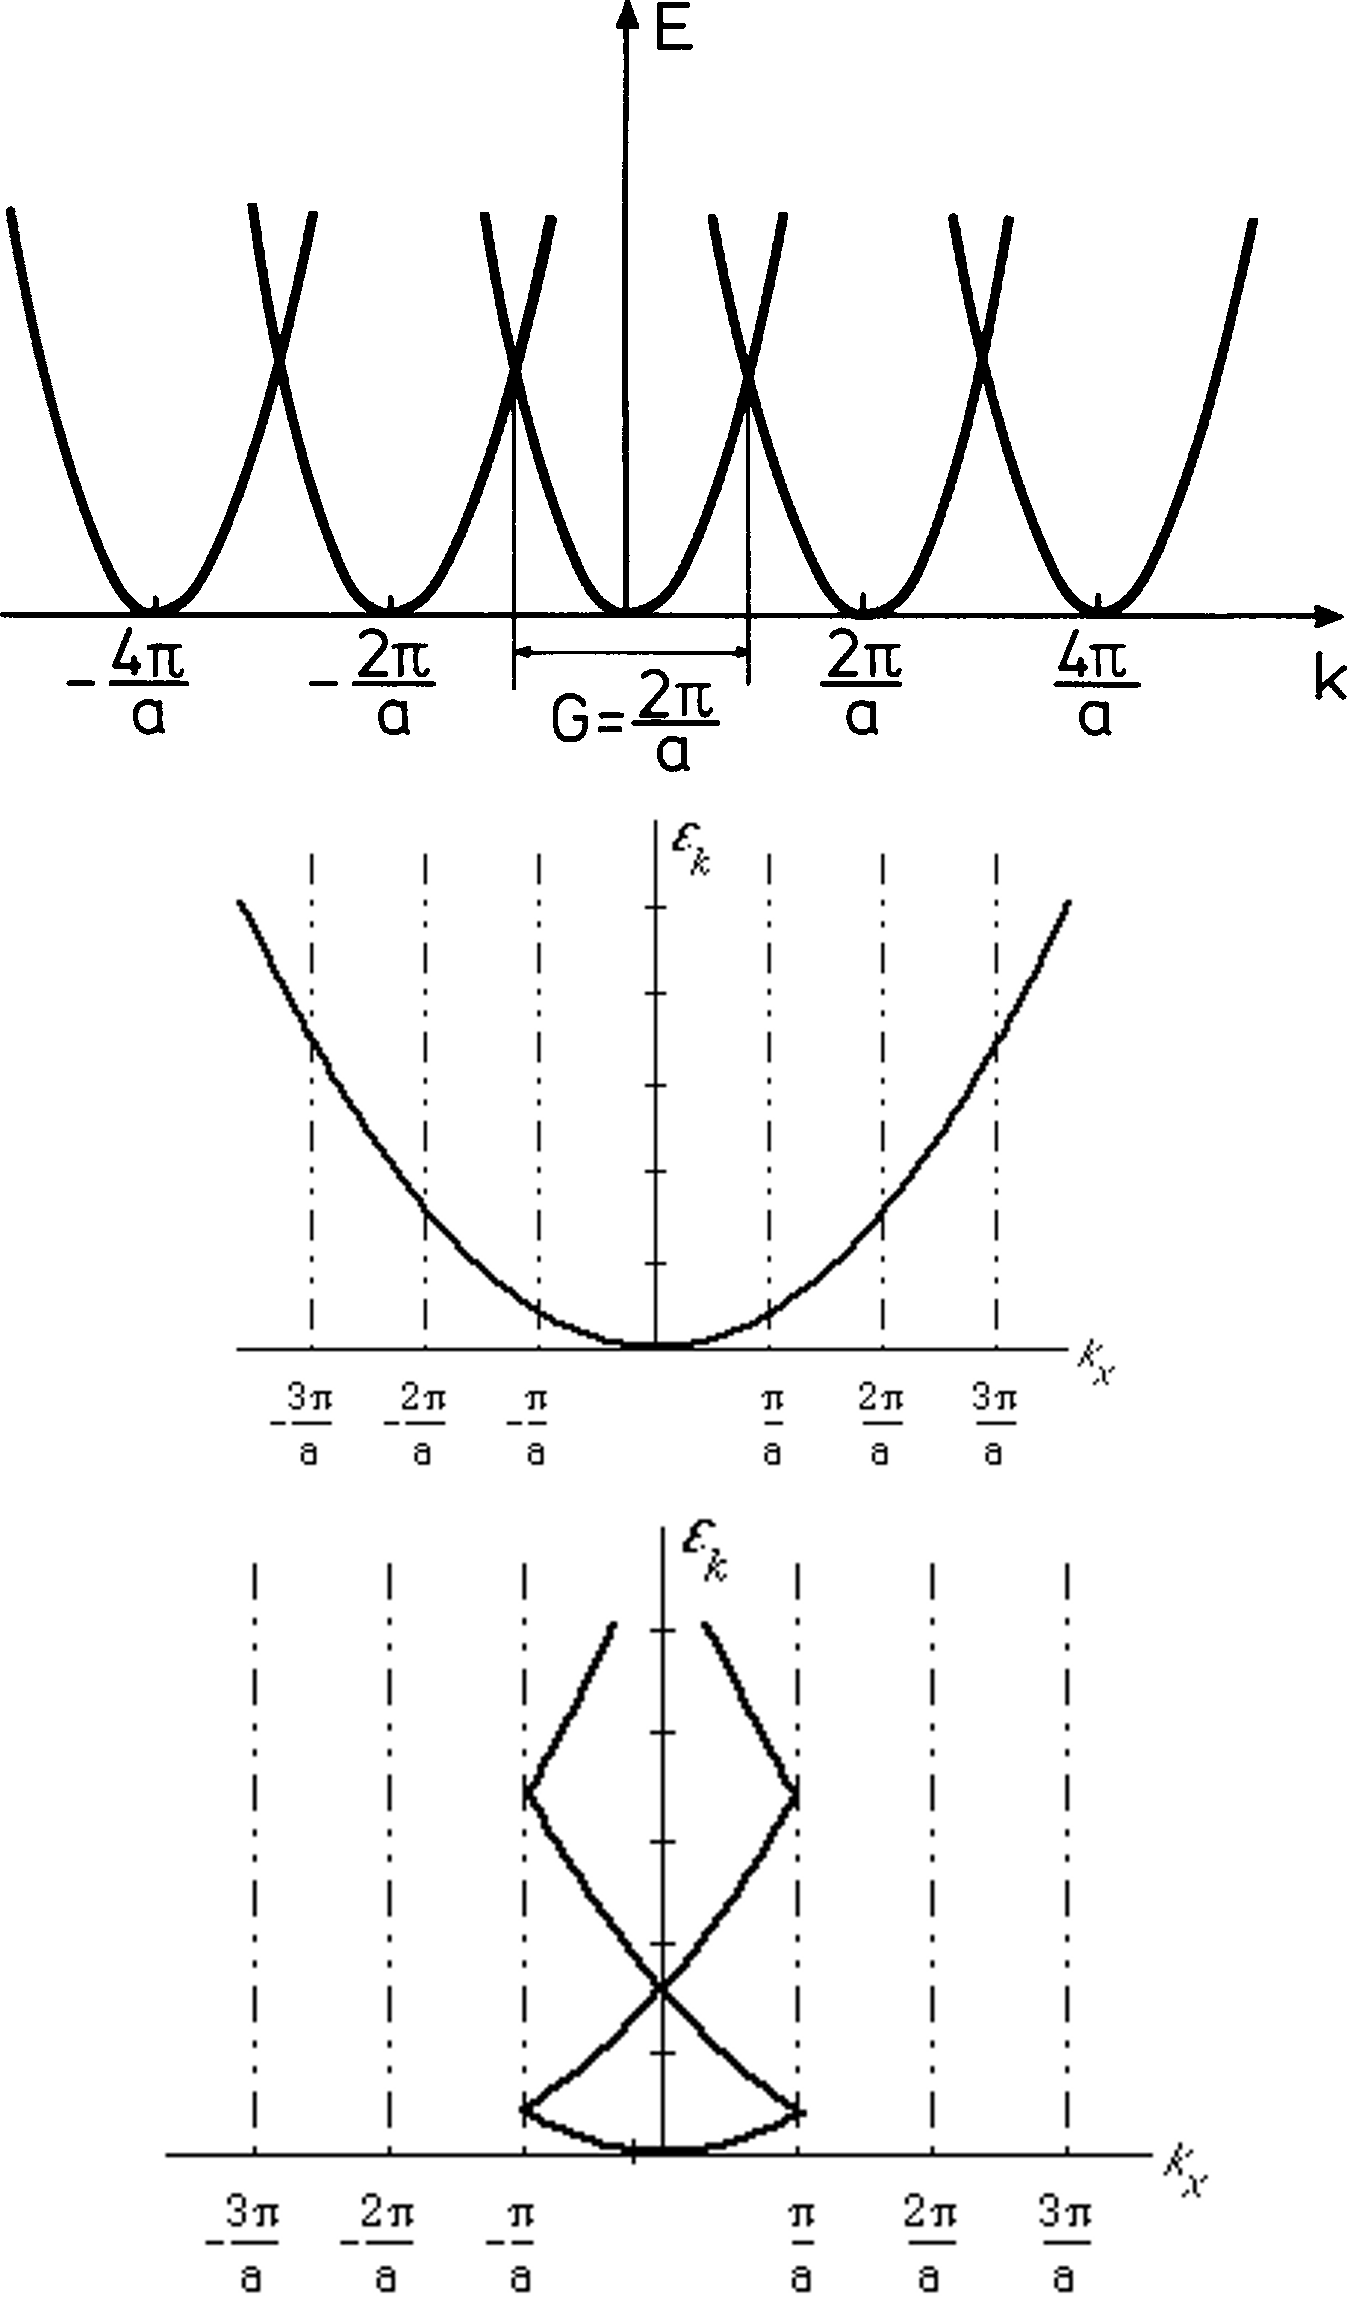
\includegraphics[width=0.8\textwidth]{figures/emptylatticeap.png}
  \caption{Representación $\varepsilon(k)$ para un
    electrón en aproximación de red vacía, caso 1D. Se muestra en
    orden ascendente el esquema de zona repetida, extendida y reducida.}
  \label{fig:emptylattice}
\end{figure}

\section{Aproximación de electrones cuasilibres}
La $k_F$ es del orden de $\nicefrac{1}{a}$ (tamaño de la PZB), así que
esperamos efectos difractivos fuertes por parte de la red. Si no nos
conformamos con la aproximación de red vacía, podemos utilizar la
teoría de perturbaciones para mejorar el modelo.
Suponemos que el potencial no es demasiado grande, y por tanto
\begin{equation}
  \varepsilon(\mathbf{k}) =  \varepsilon_\mathbf{k}^0 + \langle
  \mathbf{k} | U | \mathbf{k'}\rangle + \sum_{\mathbf{k'} \neq
    \mathbf{k}}\frac{|\langle \mathbf{k} | U |
    \mathbf{k'}\rangle|^2}{\varepsilon_\mathbf{k}^0 - \varepsilon_\mathbf{k'}^0}
\end{equation}
donde $\varepsilon_\mathbf{k}^0 =\frac{\hbar^2 k^2}{2m}$ (electrones
libres). Resolvemos el término de primer orden:
\begin{equation}
  \begin{split}
    \langle \mathbf{k} | U | \mathbf{k'}\rangle &= \frac{1}{V} \iiint
    \text{d}\mathbf{r}\ e^{-i \mathbf{k}\mathbf{r}} u(\mathbf{r}) e^{i
    \mathbf{k'} \mathbf{r}} = \\
  &= \sum_{\mathbf{G}}  \frac{1}{V} u_\mathbf{G} \iiint
  \text{d}\mathbf{r} \ e^{i [\mathbf{G} -
    (\mathbf{k}-\mathbf{k'})]\mathbf{r}} = \\
  &= u_\mathbf{G} \delta_\mathbf{G}^{\mathbf{k}-\mathbf{k'}} =
  u_\mathbf{G}, \ \ \mathbf{G}=\mathbf{k}-\mathbf{k'}
  \end{split}
\end{equation}
donde se ha utilizado que $u(\mathbf{r}) = \sum_{\mathbf{G}}
u_\mathbf{G} e^{i \mathbf{G}\mathbf{r}}$. Por tanto
\begin{equation}
  \varepsilon(\mathbf{k}) = \varepsilon_\mathbf{k}^0 +
  \cancelto{0}{U_0} + \sum_{\mathbf{k'} \neq
    \mathbf{k}}\frac{|\langle \mathbf{k} | U |
    \mathbf{k'}\rangle|^2}{\varepsilon_\mathbf{k}^0 - \varepsilon_\mathbf{k'}^0}
\end{equation}

Se ha tomado el origen de energías en el punto $\Gamma$, de forma que
$U_0 = 0$.

Tras el resultado, obtenemos algunas conclusiones:
\begin{itemize}
\item La corrección a la energía es de orden $\mathcal{O}(U^2)$. Si el
potencial es débil, la corrección es aún más débil. Obtenemos, por
tanto, una justificación del modelo de red vacía.
\item No obstante si
  $\varepsilon_\mathbf{k}^0 \sim
  \varepsilon_{\mathbf{k}-\mathbf{G}}^0$
  (frontera de PZB) la corrección diverge. Predecimos por tanto que el
  modelo de red vacía falla en la frontera.
\end{itemize}


\subsection{Demostración alternativa}
Podemos llegar a los resultados de esta sección a partir del teorema
de Bloch, sin necesidad de la teoría de perturbaciones. Utilizamos el
teorema de Bloch para escribir la función de ondas:
\begin{equation}
  \psi_\mathbf{k}(\mathbf{r}) = \sum_{\mathbf{G}}
  C_{\mathbf{k}-\mathbf{G}} e^{i(\mathbf{k}-\mathbf{G})\mathbf{r}}
\end{equation}
y despejo $C_{\mathbf{k}-\mathbf{G}}$ de la ecuación central:
\begin{equation}
  C_{\mathbf{k
    }-\mathbf{G}} = \frac{\sum_{\mathbf{G'}}
    U_{\mathbf{G'}-\mathbf{G}} C_{\mathbf{k} - \mathbf{G'}}}{\varepsilon - \varepsilon_{\mathbf{k}-\mathbf{G}}^0}
\end{equation}
Supongo que todas las $C_{\mathbf{k}-\mathbf{G}}$ son minúsculas salvo
$C_\mathbf{k}$ (en la cual $\mathbf{G}=0$), y que $\varepsilon \sim
\varepsilon_\mathbf{k}^0$. Obtengo
\begin{equation}
  C_{\mathbf{k}-\mathbf{G}} =
  \frac{U_\mathbf{-G}C_\mathbf{k}}{\varepsilon_\mathbf{k}^0 - \varepsilon^0_{\mathbf{k}-\mathbf{G}}}
\end{equation}
Tenemos una aproximación algo más restrictiva que en el modelo de red
vacía, y algo completamente equivalente a la teoría de perturbaciones
de segundo orden tras algunas transformaciones. Al despejar, obtenemos
la misma $\varepsilon(\mathbf{k})$ de antes y llegamos a las mismas
conclusiones. Para ello introducimos la $C_{\mathbf{k}+\mathbf{G}}$ hallada
en el término para $C_{\mathbf{k}+\mathbf{G}'}$ de la ecuación central
(utilizamos $\mathbf{G}=0$):

\begin{equation}
  \begin{split}
    &\left[ \frac{\hbar^2}{2m} \mathbf{k}^2 - \varepsilon
    \right] C_{\mathbf{k}} + \sum_{\mathbf{G'}}
    U_{\mathbf{G'}} C_{\mathbf{k}-\mathbf{G'}} = 0 \\
    &[\varepsilon_k^0 - \varepsilon(\mathbf{k})]C_\mathbf{k} +
    \sum_{\mathbf{G}'} U_\mathbf{G'} \frac{U_{-\mathbf{G'}}
      C_\mathbf{k}}{\varepsilon_\mathbf{k}^0 -
      \varepsilon_{\mathbf{k}-\mathbf{G'}}^0} = 0 \\
    &[\varepsilon_k^0 - \varepsilon(\mathbf{k})] \cancel{C_\mathbf{k}}+
    \sum_{\mathbf{G}'} \frac{U_{\mathbf{G'}}^2
      }{\varepsilon_\mathbf{k}^0 -
      \varepsilon_{\mathbf{k}-\mathbf{G'}}^0} \cancel{C_\mathbf{k}} = 0 \\
    &\varepsilon = \varepsilon_\mathbf{k}^0 + \sum_{\mathbf{G'}}
    \frac{U_\mathbf{G'}^2}{\varepsilon_\mathbf{k}^0 -
      \varepsilon_{\mathbf{k}-\mathbf{G'}}} 
  \end{split}
\end{equation}


\subsection{Comportamiento de la energía en la frontera}
Paso al siguiente nivel de aproximación y me quedo con los
coeficientes $\mathbf{k}-(1\mathbf{G})$, además de los
$\mathbf{k}- (0 \mathbf{G})$. La ecuación central me queda como el
siguiente sistema de dos ecuaciones:
\begin{equation}
  \begin{cases}
    (\varepsilon^0_{\mathbf{k}-\mathbf{G}})C_{\mathbf{k}-\mathbf{G}} +
    U_{-\mathbf{G}}C_\mathbf{k} + \cancel{U_0
      C_{\mathbf{k}-\mathbf{G}}} = 0 \\
    (\varepsilon_\mathbf{k}^0-\varepsilon)C_\mathbf{k} +
    \cancel{U_0 C_\mathbf{k}} +
    U_\mathbf{G}C_{\mathbf{k}-\mathbf{G}} = 0
  \end{cases}
\end{equation}
donde se ha usado que $U_0 C_{\mathbf{k}-\mathbf{G}} = U_0
C_\mathbf{k} \stackrel{\text{def}}{=} 0$. Tengo dos ecuaciones con dos
incógnitas, como quiero que no tengan una
solución trivial impongo un determinante nulo:
\begin{equation}
  \begin{vmatrix}
    \varepsilon_\mathbf{k}^0 - \varepsilon & U_\mathbf{G} \\
    U_{-\mathbf{G}} & \varepsilon_{\mathbf{k}-\mathbf{G}}^0 - \varepsilon
  \end{vmatrix} = 0
\end{equation}
Resolviendo (recordar que $U_\mathbf{G} = U_\mathbf{G}^*$) obtenemos
\begin{equation}
  \varepsilon = \frac{\varepsilon_\mathbf{k}^0 +
    \varepsilon_{\mathbf{k}-\mathbf{G}}^0}{2} \pm \sqrt{\left(
      \frac{\varepsilon_\mathbf{k}^0 -
        \varepsilon_{\mathbf{k}-\mathbf{G}}^0}{2} \right)^2 + |U_\mathbf{G}|^2}
\end{equation}
En el caso $|\mathbf{k}| = |\mathbf{k}-\mathbf{G}|$ tenemos que
$\varepsilon_\mathbf{k}^0 = \varepsilon_{\mathbf{k}-\mathbf{G}}^0$ y
por tanto
\begin{equation}
  \varepsilon = \varepsilon_\mathbf{k}^0 \pm |U_\mathbf{G}|
\end{equation}
En la figura \ref{fig:energygap} puede verse esta diferencia de
energía de valor $2|U_\mathbf{G}|$ y la forma funcional de $\varepsilon(\mathbf{k})$.
\begin{figure}
  \centering
  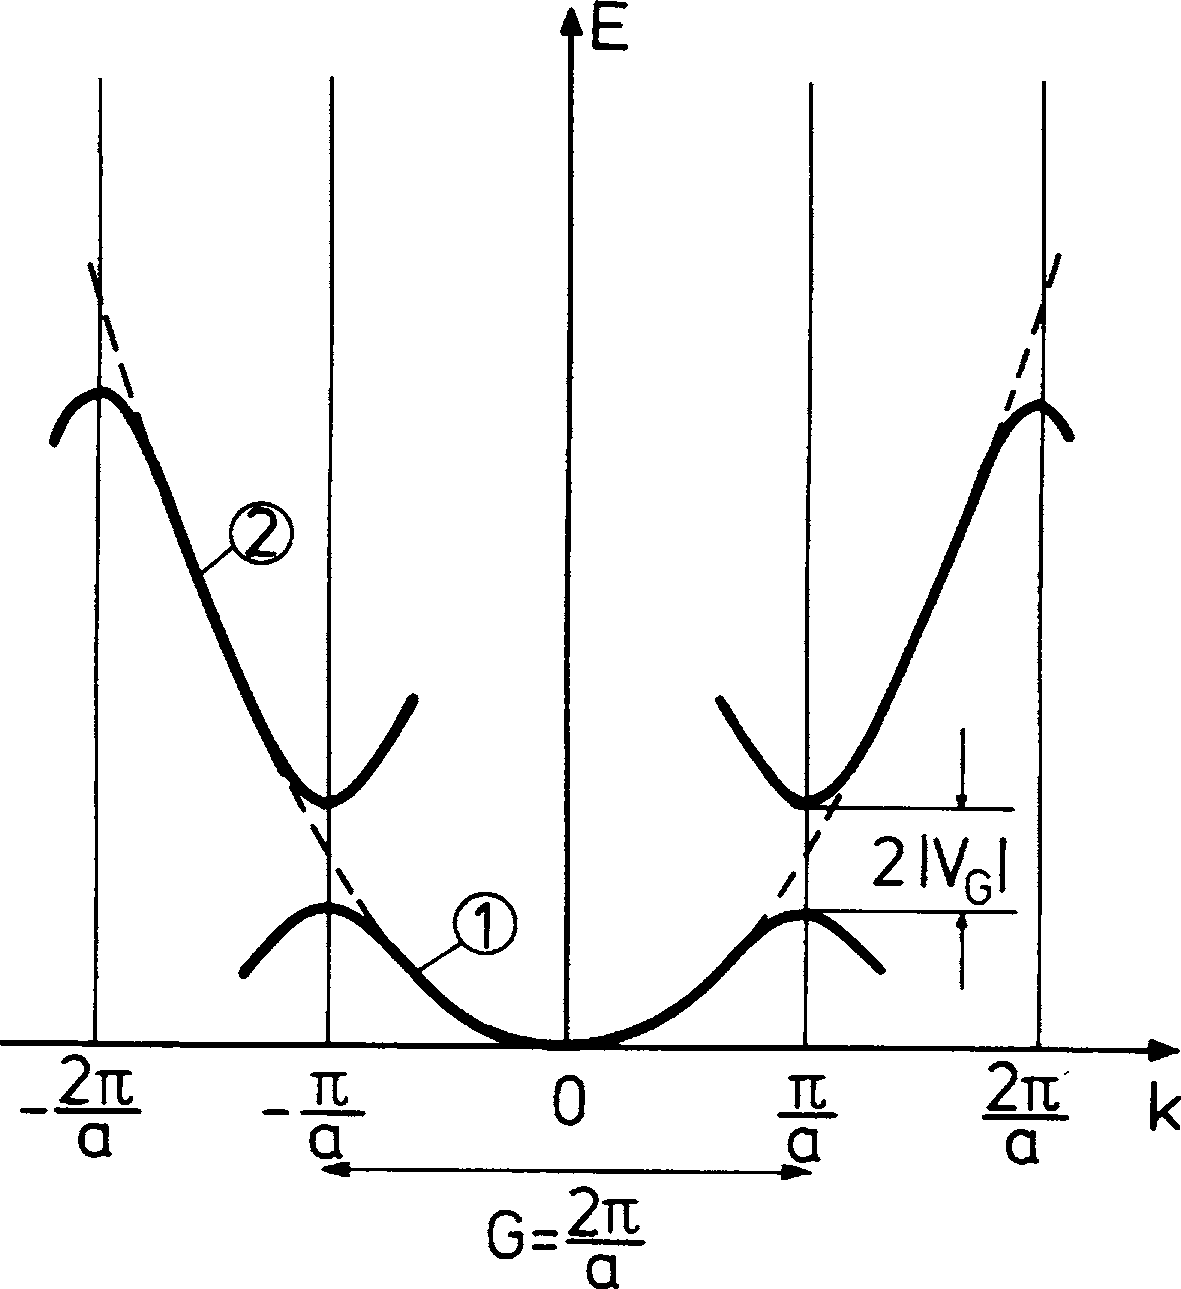
\includegraphics[width=0.8\textwidth]{figures/energygap.png}
  \caption{Forma funcional de la energía en la aproximación de
    electrones cuasilibres tras la corrección en la frontera
    resultante de usar dos coeficientes. En línea discontinua se muestra el caso de
  electrones libres.}
  \label{fig:energygap}
\end{figure}

Con la ecuación central podemos hallar las funciones de
onda\footnote{La notación $\psi^\pm$ indica la simetría de la onda al
  cambiar $x$ por $-x$.} de cada
rama en los puntos degenerados ($\mathbf{k}$ en frontera de
PZB). Supongamos que el potencial es positivo (si no simplemente la
$\psi^+$ se intercambia con la $\psi^-$), y resolvamos para la rama
de $\psi^-$ la ecuación central (recordemos que para la frontera
$\varepsilon = \varepsilon_\mathbf{k}^0 \pm |U_\mathbf{G}|$):
\begin{equation}
  \begin{split}
    (\varepsilon_\mathbf{k}^0 - \varepsilon^+) C_\mathbf{k} +
    U_\mathbf{G} C_{\mathbf{k}-\mathbf{G}} &= 0 \\
    ( \cancel{\varepsilon_\mathbf{k}^0}-  \cancel{\varepsilon_\mathbf{k}^0}- |U_\mathbf{G}|) C_\mathbf{k} +
    U_\mathbf{G} C_{\mathbf{k}-\mathbf{G}} &= 0 \\
\frac{C_\mathbf{k}}{C_{\mathbf{k}-\mathbf{G}}} =
\frac{U_\mathbf{G}}{|U_\mathbf{G}|} = \text{sgn} (U_\mathbf{G}) > 0
  \end{split}
\end{equation}
obtengo que
\begin{equation}
  \psi^+ \propto e^{i \mathbf{k}\mathbf{r}} + e^{i
    (\mathbf{k}-\mathbf{G}) \mathbf{r}} \ \rightarrow \ |\psi^-|^2
  \propto \cos^2 \frac{\mathbf{G}\mathbf{r}}{2} \tag{S wave}
\end{equation}
Repitiendo las cuentas para la rama de $\psi^-$ obtengo

\begin{equation}
  \psi^- \propto e^{i \mathbf{k}\mathbf{r}} - e^{i
    (\mathbf{k}-\mathbf{G}) \mathbf{r}} \ \rightarrow \ |\psi^-|^2
  \propto \sin^2 \frac{\mathbf{G}\mathbf{r}}{2} \tag{P wave}
\end{equation}
Notar que sólo han aparecido dos puntos degenerados por haber sido el
problema tratado en 1D. En N dimensiones pueden aparecer muchos más
puntos degenerados, con varios cruces en ellos y determinantes más grandes.

\section{Tight binding}
Existen muchos métodas para resolver las bandas de un sólido. Una vez
visto el extremo de electrones cuasilibres, es interesante ver el
ejemplo opuesto, electrones muy ligados a sus iones, siendo sus $\psi$
prácticamente los orbitales del átomo libre. A esta aproximación se le
denomina \emph{tight binding}. De forma matemática,
\begin{equation}
  \mathcal{H} \sim \mathcal{H}_\text{atomic}, \ \
  \mathcal{H}_\text{at} \phi_n = \varepsilon_n \phi_n
\end{equation}
donde las $\phi_n (\mathbf{r}-\mathbf{R})$ corresponden a los distintos orbitales atómicos del
átomo libre. Suponemos una colectividad de átomos con los niveles
atómicos como espectro energético, sin influenciarse entre ellos.

Queremos resolver $\mathcal{H}$, donde $\mathcal{H} \phi = \varepsilon
\phi$. Lo escribimos como
\begin{equation}
  \mathcal{H} = \mathcal{H}_\text{at} + \Delta U(\mathbf{r})
\end{equation}
con $\Delta U$ el potencial de la red menos el potencial atómico. Esta
forma de expresar $\mathcal{H}$ es más útil que la clásica
$\mathcal{H} = E_c + E_p$, como veremos. Presuponemos\footnote{Wannier
  demostró que tada función Bloch se puede estribir como en nuestra
  suposición, así que no estamos eliminando ningún grado de libertad.} una forma para
las funciones de onda del tipo:
\begin{equation}
  \psi(\mathbf{r}) = \sum_{\mathbf{R}} e^{i \mathbf{k} \mathbf{r} } \phi(\mathbf{r}-\mathbf{R})
\end{equation}
con $\phi(\mathbf{r}) = \sum_{n} b_n \phi_n(\mathbf{r})$ combinación
lineal de orbitales atómicos. Nos queda
\begin{equation}
  [\mathcal{H}_\text{at} + \Delta U(\mathbf{r})] \psi = \varepsilon \psi
\end{equation}

Para sacar la energía, Ashcroft multiplica por un orbital atómico
$\phi_m^* (\mathbf{r})$ e integra (básicamente, proyecta sobre dicho
orbital):
\begin{equation}
\begin{split}
  \iiint \text{d}\mathbf{r}\ \phi_m^* (\mathcal{H}_\text{at} + \Delta
  U) \psi &= \varepsilon(\mathbf{k}) \iiint \text{d}\mathbf{r} \
  \phi_m^* \psi \\
  \iiint \text{d} \mathbf{r}\ \underbrace{\phi_m^*
  \mathcal{H}_\text{at}}_{\varepsilon_m \phi_m^*}\psi +
  \iiint \text{d}\mathbf{r}\ \phi_m^* \Delta U \psi &= \varepsilon(\mathbf{k}) \iiint \text{d}\mathbf{r} \
  \phi_m^* \psi \\
  \iiint \text{d}\mathbf{r} \ \phi_m^* \Delta U \psi &= (\varepsilon -
  \varepsilon_m) \iiint \text{d}\mathbf{r} \ \phi^*_m \psi
\end{split}
\end{equation}
Resuelvo ambas integrales:
\begin{itemize}
\item Para la primera obtengo
\begin{equation}
  \iiint \text{d} \mathbf{r} \ \phi_m^* (\mathbf{r}) \psi(\mathbf{r})
  = \sum_{\mathbf{R}} e^{i \mathbf{k}\mathbf{R}} \sum_{n} b_n \iiint
  \text{d}\mathbf{r} \ \phi_m^* (\mathbf{r}) \phi_n
  (\mathbf{r}-\mathbf{R}) = \cdots
\end{equation}
separando el caso $\mathbf{R} = \mathbf{0}$,
\begin{equation}
  \begin{split}
  \cdots &= \sum_{n} b_n \iiint \text{d} \mathbf{r} \
  \phi_m^*(\mathbf{r})\phi_n(\mathbf{r}) + \\ &+
\sum_{\mathbf{R}\neq 0} e^{i \mathbf{k}\mathbf{R}}\sum_{n} b_n \iiint
\text{d} \mathbf{r} \ \phi_m^*(\mathbf{r})\phi_n(\mathbf{r} - \mathbf{R})
  \end{split}
\end{equation}
como los orbitales atómicos son ortogonales,
$\iiint \text{d}\mathbf{r}\ \phi_m^* \phi_n = \delta_n^m$, siendo el
primer sumando $\sum_{n} b_n \delta_n^m = b_m$.
\item La segunda integral queda como
\begin{equation}
  \begin{split}
  \iiint &\text{d}\mathbf{r}\ \phi_m^* (\mathbf{r}) \Delta
  U(\mathbf{r}) \sum_{\mathbf{R}} e^{i \mathbf{k}\mathbf{r}} \sum_{n}
  b_n \phi_n (\mathbf{r}-\mathbf{R}) =   \\ &= \sum_{n}b_n \iiint
  \text{d}\mathbf{r} \phi_m^* (\mathbf{r}) \Delta U (\mathbf{r})
  \phi_m (\mathbf{r})    + \\ &+     \sum_{\mathbf{R}\neq 0} e^{i \mathbf{k}
    \mathbf{R}} \sum_{n} b_n \iiint \text{d}\mathbf{r} \ \phi_m^*
  (\mathbf{r}) \Delta U (\mathbf{r}) \phi_n (\mathbf{r}-\mathbf{R})
  \end{split}
\end{equation}
\end{itemize}

Ya sólo resta introducir las ecuaciones en un ordenador y resolverlas
numéricamente. Es un método computacionalmente eficaz, funciona bien
en aislantes y semiconductores y falla un poco en metales.

\subsection{Aplicación en electrones s}
En este caso el set de coeficientes sólo tiene un miembro,
$\{b_n\} = b_s$, y sin degeneración (los orbitales s no lo están):
\begin{equation}
  \psi(\mathbf{r}) = \sum_{n}e^{i \mathbf{k}\mathbf{R}} b_s \phi_s (\mathbf{r}-\mathbf{R})
\end{equation}
Tenemos que resolver una única ecuación. Los electrones p nos darían
un sistema de tres ecuaciones, los d cinco, etc.

\begin{equation}
\begin{split}
  &b_s \iiint \text{d}\mathbf{r}\ \phi_s^* (\mathbf{r}) \Delta
  U(\mathbf{r}) \phi_s (\mathbf{r}) + \\ &+ \sum_{\mathbf{R}\neq 0} e^{i
    \mathbf{k}\mathbf{R}} b_s \iiint \text{d}\mathbf{r}\ \phi_s^*
  (\mathbf{r}) \Delta U (\mathbf{r}) \phi_s (\mathbf{r}-\mathbf{R}) =
  \\
&= (\varepsilon (\mathbf{k}) - \varepsilon_s) [b_s +
\sum_{\mathbf{R}\neq 0} e^{i \mathbf{k} \mathbf{R}} b_s \iiint
\phi_s^* (\mathbf{r}) \phi_s (\mathbf{r}-\mathbf{R})]
\end{split}
\end{equation}
La única incógnita es la $\varepsilon(\mathbf{k})$, que es lo que
busco. Tengo tres integrales a resolver:
\begin{itemize}
\item La última integral corresponde al solapamiento de las funciones
  de distintos átomos. Es muy pequeña por la suposición inicial del
  modelo de tight binding.
\begin{equation}
  \alpha(\mathbf{R}) = \iiint \text{d}\mathbf{r}\ \phi^* (\mathbf{r})
  \phi(\mathbf{r}-\mathbf{R}) \ \sim 0
\end{equation}
\item Salvo un signo menos \emph{ad hoc} para que resulte positiva (ya
  que $\Delta U < 0$) la primera integral corresponde al valor medio
  del potencial corregido en cada punto de la red. Es muy pequeña
  porque $\Delta U$ es el potencial total menos el atómico, y hemos
  supuesto que el atómico es la parte más representativa del potencial
  total, siendo la corrección $\Delta U$ pequeña.
  \begin{equation}
    \beta = - \iiint \text{d}\mathbf{r}\
    |\phi(\mathbf{r})|^2 \Delta U (\mathbf{r}) \ \sim 0
  \end{equation}
\item Por último, la primera de todas las integrales tiene un
  significado similar a $\beta$, pero en dos puntos de la red. Si
  fuera nula, estamos suponiendo átomos aislados, y no estamos
  interesados en llevar la aproximación tan lejos. El signo menos está
  por las mismas razones que el de $\beta$.
  \begin{equation}
   \gamma (\mathbf{R}) = - \iiint \text{d}\mathbf{r}\ \phi^* (\mathbf{r}) \Delta U \phi(\mathbf{r}-\mathbf{R})
  \end{equation}
\end{itemize}

Con estas definiciones obtenemos la siguiente fórmula para la energía:
\begin{equation}
  \boxed{
   \varepsilon(\mathbf{k}) = \varepsilon_s - \frac{\displaystyle \beta +
    \sum_{\mathbf{R}\neq 0}\gamma(\mathbf{R}) e^{i
      \mathbf{k}\mathbf{R}}}{\displaystyle 1 + \sum_{\mathbf{R}\neq 0}
    \alpha(\mathbf{R})e^{i \mathbf{k}\mathbf{R}}}
  } \tag{s band energy}
\end{equation}

Ahora, aproximemos. Sabemos que $\phi(\mathbf{r})$ es real (es una
función del tipo del orbital s) y sólo depende de $|\mathbf{r}|$ (por
el mismo motivo):
\begin{equation}
  \phi (\mathbf{r}) = f(r) \in \mathbb{R}
\end{equation}
Respecto al potencial, $\Delta U(\mathbf{r}) \in \mathbb{R}$ y por su
simetría de inversión $ \Delta U (\mathbf{r}) =
  \Delta U(- \mathbf{r})$ lo que implica que $\gamma(\mathbf{R}) =
  \gamma(-\mathbf{R})$.

Eliminando $\alpha$ obtenemos:
\begin{equation}
  \varepsilon(\mathbf{k}) \sim \varepsilon_s - \beta -
  \sum_{\mathbf{R}\neq 0} \gamma(\mathbf{R}) e^{i \mathbf{k}
    \mathbf{R}} \sim \varepsilon_s - \beta - 2\gamma \sum_{\text{n.n.}>0} \cos
  (\mathbf{k} \mathbf{R})
\end{equation}
donde ``$ \text{n.n.}> 0$'' denota sumar a primeros vecinos positivos. Notar el dos,
implicando que por la simetría de $\gamma$ sólo sumamos los vecinos de
``un lado''. Vemos que $\gamma$ nos da el ancho de banda (es la
amplitud de una función coseno) y $\beta$ un
decrecimiento de la energía. Notar que puede existir solapamiento
entre bandas si su ancho es suficiente.

\subsubsection{Ejemplo: Estructura SC}
Hay 6 primeros vecinos, pero sólo usaremos 3 para poder emplear la
fórmula vista para bandas s (el factor 2 que tiene arregla este
hecho). De las 6 posibles $\mathbf{k}\mathbf{R}$, empleamos sólo las
positivas:
\begin{equation}
  \mathbf{k}\mathbf{R} =
  \begin{cases}
    &\pm k_x a \\
    &\pm k_y a \\
    &\pm k_z a \\
  \end{cases}
\end{equation}
La energía de las bandas s es por tanto
\begin{equation}
  \varepsilon(\mathbf{k}) = \varepsilon_s - \beta - 2\gamma [\ \ \cos(k_x
  a) + \cos(k_y a) + \cos(k_z a)\ \ ]
\end{equation}
Como $\varepsilon$ va desde $\varepsilon_s - \beta - 6\gamma$ hasta
$\varepsilon_s - \beta + 6\gamma$, el ancho de bando es $\Delta
\varepsilon = 12\gamma$. Si $\mathbf{k}\mathbf{R}$ es muy pequeño se
tiene que
\begin{equation}
  \begin{split}
  \varepsilon (\mathbf{k}) &\sim \varepsilon_s - \beta - 2\gamma \left[
    \sum_{i=1}^3 \left( \frac{1}{2}(k_{x_i} a)^2 + 1 \right) \right] =
  \\ &= \varepsilon_s - \beta - 6\gamma - \gamma k^2 a^2
  \end{split}
\end{equation}
Por tanto, comprobamos como para bajos $\mathbf{k}$ recuperamos la
aproximación parabólica. La discrepancia está en la forma funcional de
la energía más allá, que deja de ser parabólica y se aplana.

\section{Bandas en metales, semiconductores y aislantes}
En el siguiente capítulo veremos que una banda llena es aislante;
siendo $N$ el número de celdas primitivas del cristal, en una banda
caben $2N$ electrones (uno con cada espín). Según el número de
electrones de valencia del metal, podemos hacer una primera
clasificación del sólido:

\begin{itemize}
\item Es tentador decir que si el sistema tiene un número
  impar de electrones es imposible llenar todas las bandas y estamos
  ante un conductor. Notar que este argumento supone que todos los
  electrones de valencia participan en la conducción, pero es una
  aproximación útil.
\item Si el número de electrones es par, es sistema debería ser
  aislante. Se está presuponiendo que no hay solapamiento entre
  bandas, lo cual ocurre en algunos metales. Si existe solapamiento,
  estaremos ante un aislante o un semiconductor.
\end{itemize}

En función del solapamiento de las bandas, podemos ver las propiedades
aislantes o metálicas de un sólido (fig. \ref{fig:bandclasification} y
\ref{fig:bandfill}).
\begin{figure}
  \centering
  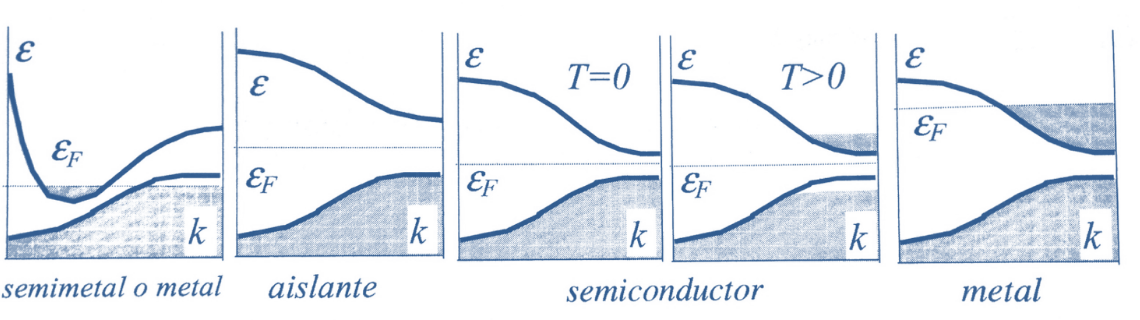
\includegraphics[width=0.8\textwidth]{figures/bandclasification.png}
  \caption{Según el solapamiento entre bandas (figura superior)
    tenemos distintas propiedades en el sólido.}
  \label{fig:bandclasification}
\end{figure}

\begin{figure}
  \centering
  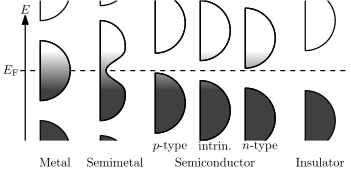
\includegraphics[width=0.8\textwidth]{figures/bandfill.png}
  \caption{Filling of the electronic states in various types of
    materials at equilibrium. Here, height is energy while width is
    the density of available states for a certain energy in the
    material listed. The shade follows the Fermi–Dirac distribution
    (black=all states filled, white=no state filled). In metals and
    semimetals the Fermi level EF lies inside at least one band. In
    insulators and semiconductors the Fermi level is inside a band
    gap; however, in semiconductors the bands are near enough to the
    Fermi level to be thermally populated with electrons or holes.}
  \label{fig:bandfill}
\end{figure}



\subsection{Ejemplos de aplicación de los modelos}

\paragraph{Aluminio}
Tiene una estructura FCC y una configuración electrónica del tipo
[Ne]3s\textsuperscript 2 3p\textsuperscript 1. En teoría debería ser
un metal (y en efecto, lo es). En la figura \ref{fig:alexample} pueden
verse su esfera de Fermi y su estructura de bandas.


Los metales alcalinos también tienen un buen ajuste, pero su esfera de
Fermi queda justo dentro de la primera zona de Brillouin. Por tanto,
junto al aluminio, son buenos candidatos a ser modelados por
electrones cuasilibres.
\begin{figure}
  \centering
  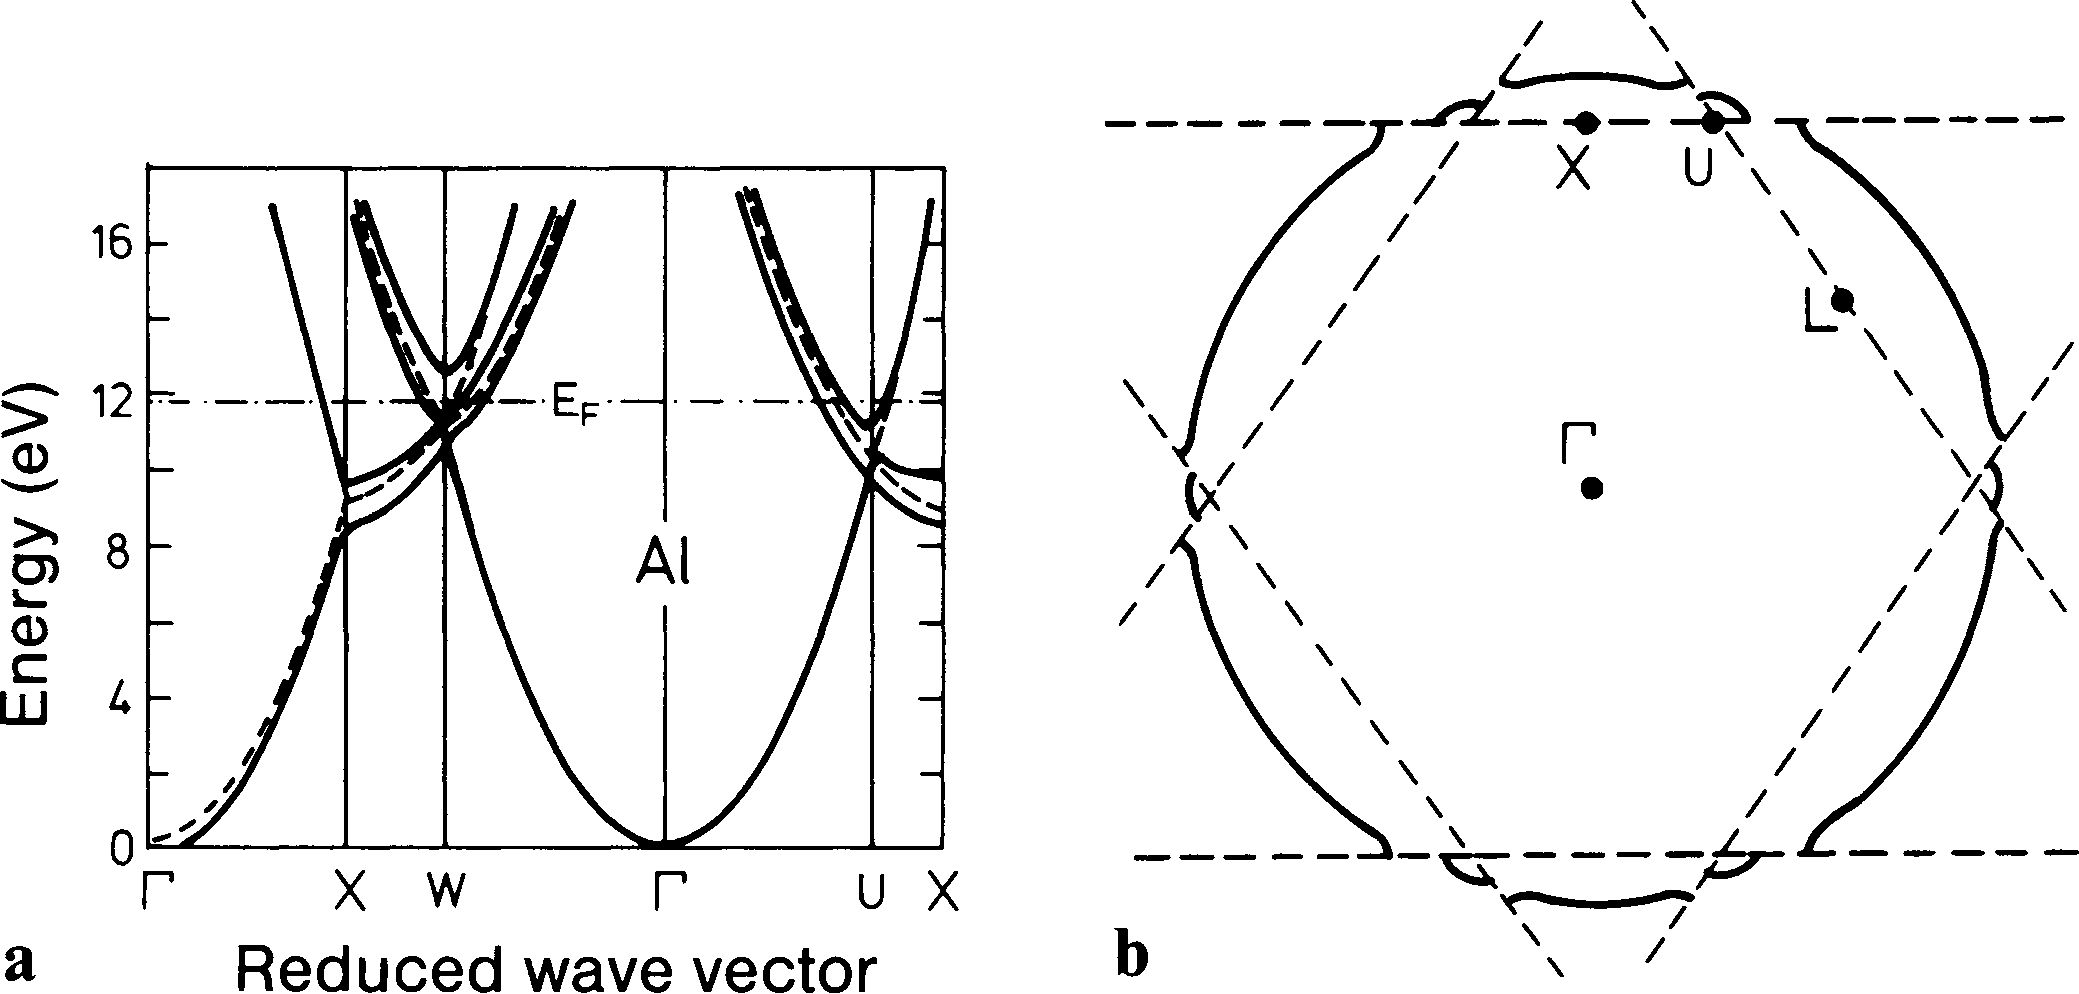
\includegraphics[width=0.8\textwidth]{figures/alexample.png}
  \caption{En la figura \emph{a} podemos ver la estructura de bandas
    teórica del aluminio. Notar como la aproximación de celda vacía
    (línea discontínua funciona bien. En la dirección
    $\Gamma \text{X} $ podemos ver un claro gap tras la parábola. En
    \emph{b} vemos como la esfera de Fermi del alumínio (línea sólida)
    sobrepasa el corte mostrado de la primera zona de Brillouin.}
  \label{fig:alexample}
\end{figure}

\paragraph{Cobre} Su estructura también predice un observable aspecto
metálico ([Ar]3d\textsuperscript {10} 4s\textsuperscript 1). Cuando
observamos las bandas (fig. \ref{fig:cuexample}), comprobamos que las
bandas s sí que se ajustan bien a un modelo de electrones cuasilibres;
no así las p que tienen una relación de dispersión casi plana. El
modelo de tight binding predice que bandas muy estrechas tienen poco
solapamiento; podemos ver esto en como los electrones d del cobre (los
cuales tienen bandas muy estrechas, casi son deltas de Dirac) tienen
están muy localizados en la densidad de estados.

\begin{figure}
  \centering
  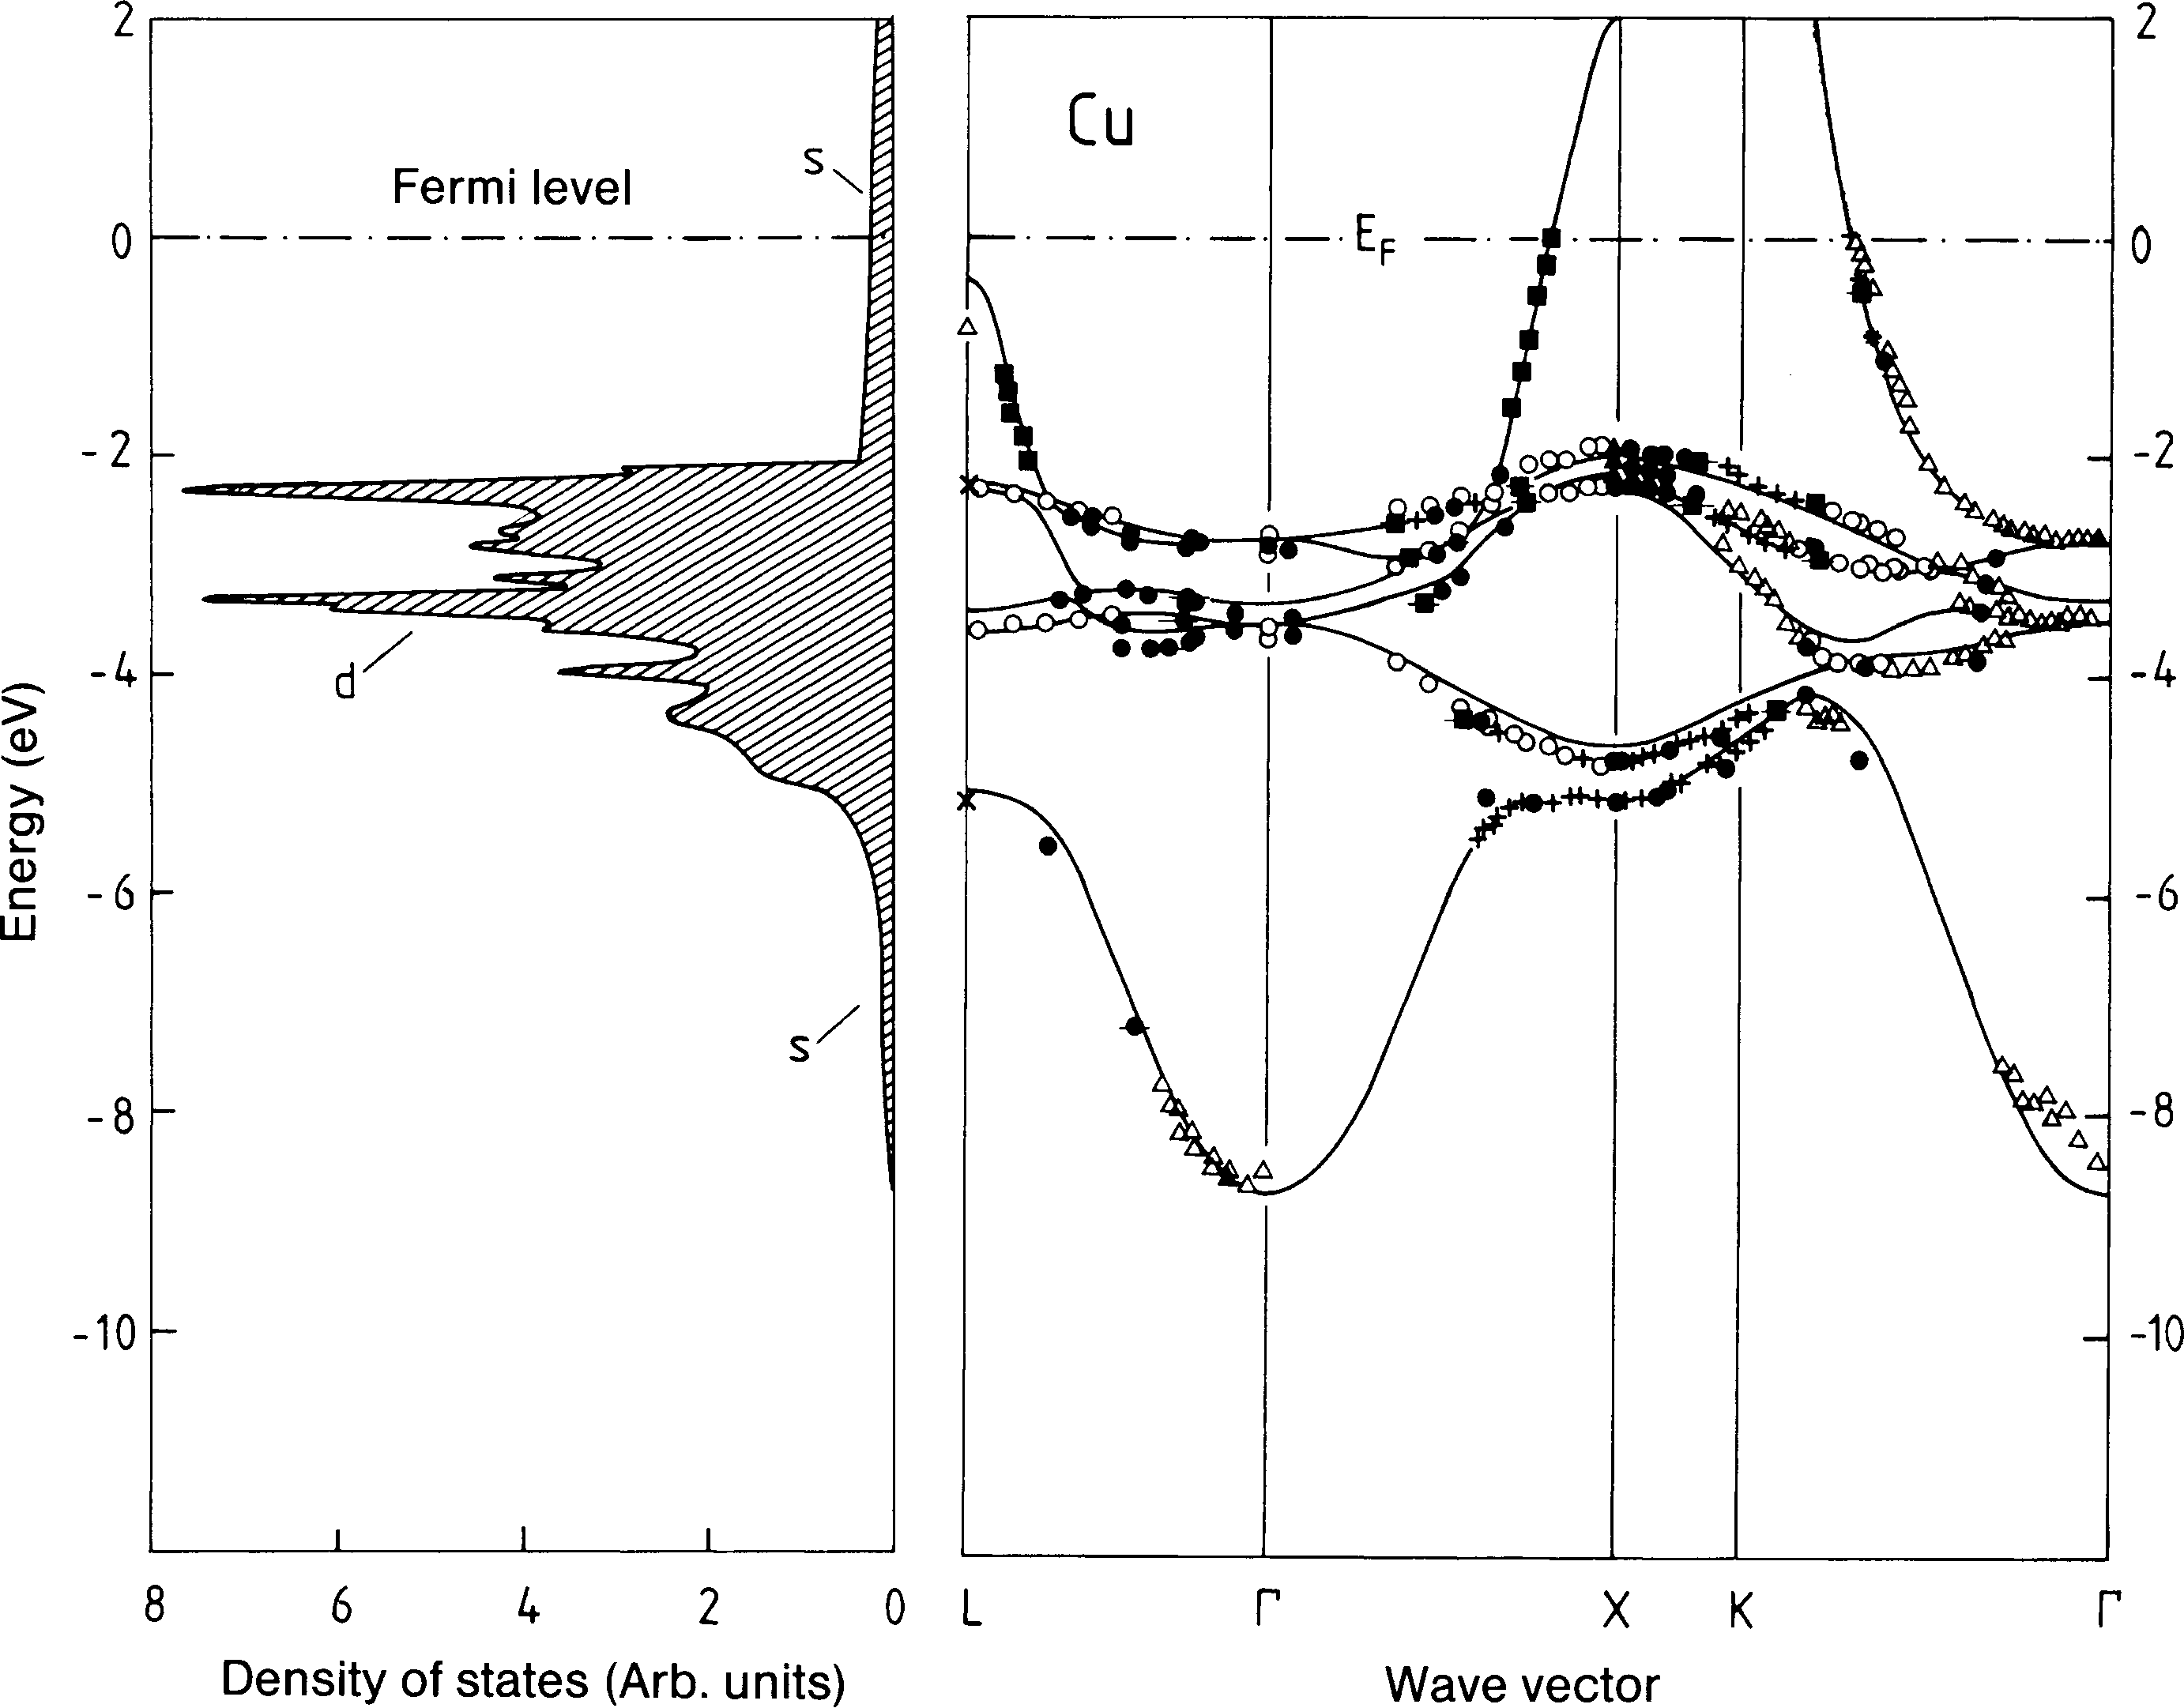
\includegraphics[width=0.8\textwidth]{figures/cuexample.png}
  \caption{Curvas de dispersión $\varepsilon(\mathbf{k})$ para el
    cobre. Vemos como las relaciones de dispersión de las bandas s se
    ajustan bien a un modelo de electrones cuasilibres pero las p
    no. Notar como la densidad de estados muestra una gran
    localización de los electrones d en la densidad de estados.}
  \label{fig:cuexample}
\end{figure}

\paragraph{Germanio}
Su estructura electrónica es [Ar]3d\textsuperscript {10}
4s\textsuperscript 2 4p\textsuperscript 2, tiene una estructura
cristalina como la del diamante. Según las reglas vistas anteriormente
debería ser aislante (no es el caso) o semiconductor. La estructura de
bandas (fig. \ref{fig:geexample}) indica que es un semiconductor por
lo pequeño del gap en las bandas.

\begin{figure}
  \centering
  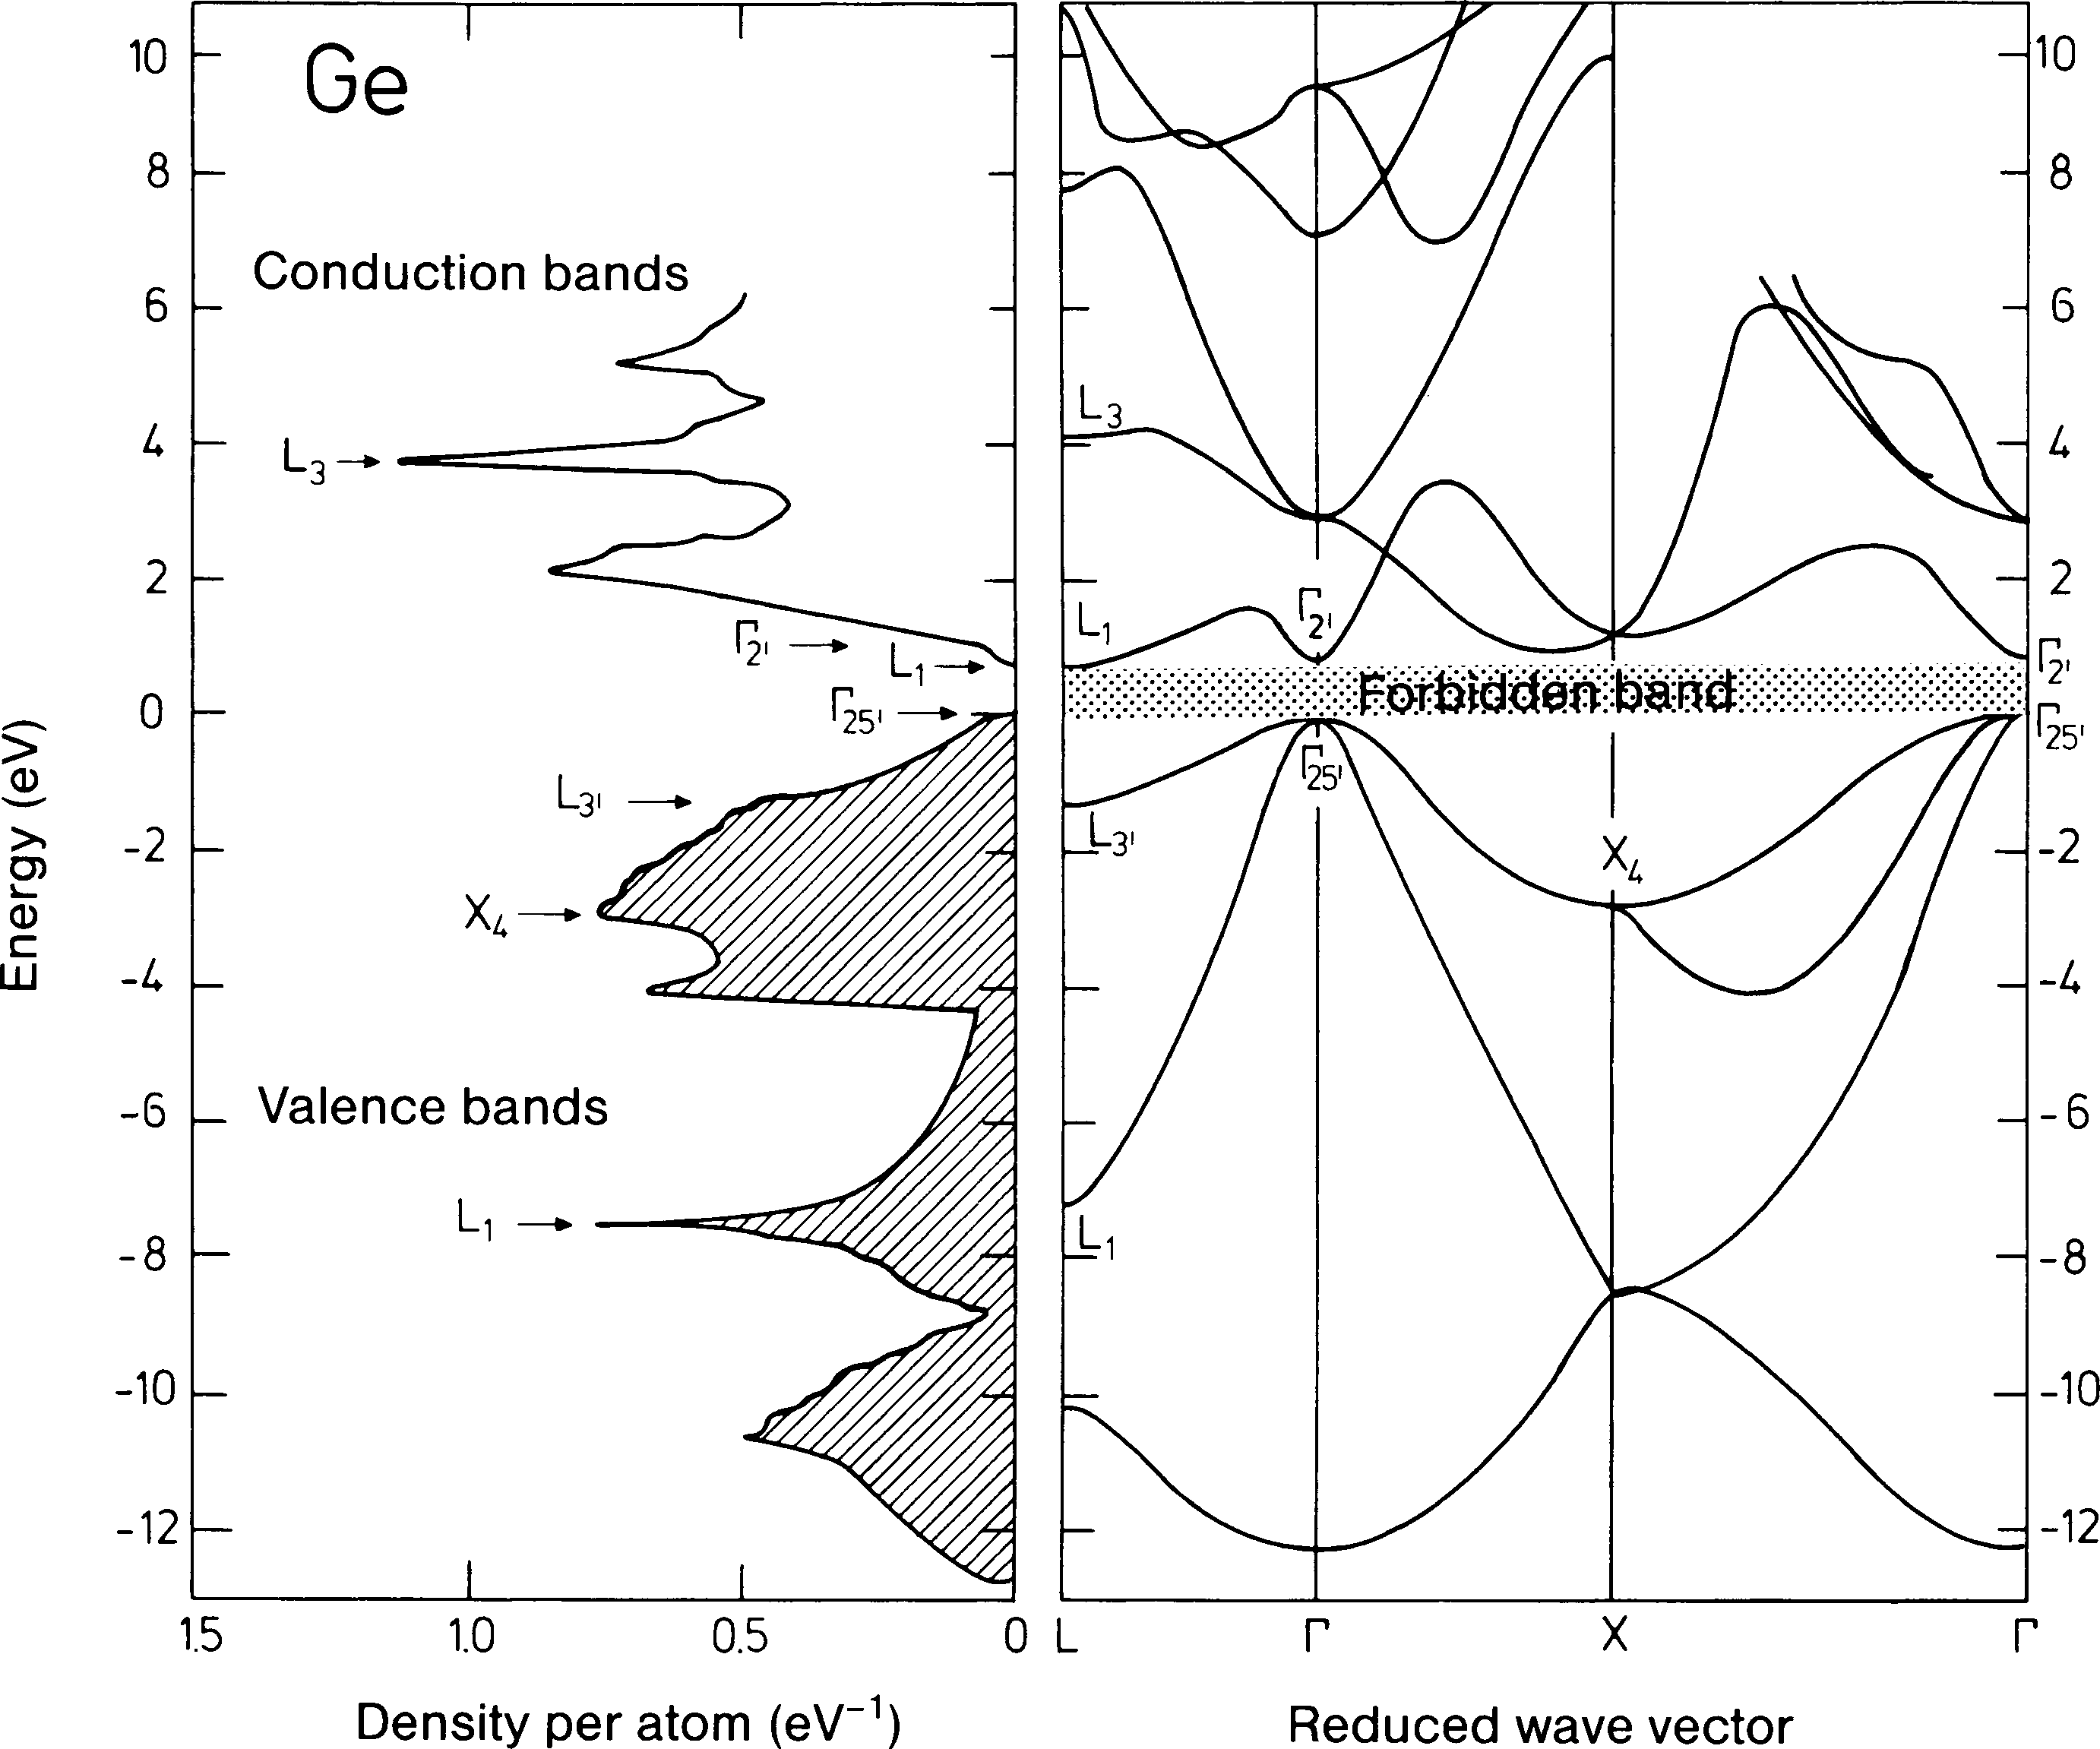
\includegraphics[width=0.8\textwidth]{figures/geexample.png}
  \caption{Estructura de bandas del germanio. El nivel de Fermi está
    situado en el origen de energías. Notar como el gap marcado es
    absoluto; en \SI{-10}{\eV} podemos ver un gap para $\Gamma \text
    L$ que no lo es para $\Gamma \text X$. Notar las singularidades
    de Van Hoff cuando se aplana la relación de dispersión (puntos
    L\textsubscript 1 y L\textsubscript 3, por ejemplo).}
  \label{fig:geexample}
\end{figure}

\chapter{Dinámica semiclásica de electrones Bloch}
\section{Teorema de la masa efectiva}
El concepto de masa efectiva es algo que ya vimos en
\ref{subsec:accurate}; en este capítulo se verá de manera más detallada.

Sea una función de Bloch tal que
\begin{equation}
  \psi_{n \mathbf{k}} (\mathbf{r}) = e^{i \mathbf{k}\mathbf{r}} u_{n
    \mathbf{k}} (\mathbf{r})
\end{equation}
Si la sustituímos en la ecuación de Schrodinger ($\mathcal{H} \psi_{n
  \mathbf{k}} = \varepsilon_n \psi_{n \mathbf{k}}$) obtenemos $\mathcal{H}_\mathbf{k} u_{n
  \mathbf{k}} = \varepsilon_n u_{n \mathbf{k}}$. Notando que $\nabla^2
(fg) = f \nabla^2 g + g \nabla^2 g + 2 \nabla f \nabla g$ podemos
escribir dicho hamiltoniano como 
\begin{equation}
  \mathcal{H}_\mathbf{k} = \frac{-\hbar^2}{2m}\nabla^2 + \frac{\hbar^2
  k^2}{2m} + \frac{\hbar}{m}\mathbf{k}(-i \hbar \nabla) + U(\mathbf{r})
\end{equation}
No es más que el hamiltoniano original modificado con $\mathcal{H}' =
\frac{\hbar^2 k^2}{2m} + \frac{\hbar}{m}(-i \hbar \nabla)$, de forma
que $\mathcal{H}_\mathbf{k} = \mathcal{H}_0 + \mathcal{H}' =
\mathcal{H}_0 + \left[ \frac{\hbar^2 k^2}{2m} - \frac{\hbar}{m} \mathbf{K}\mathbf{P} \right]$.

Una posible solución al problema es suponer que $\mathcal{H}' l
\mathcal{H}_0$ y utilizar la teoría de perturbaciones (método
$\mathbf{K}\mathbf{P}$). Aquí se utilizará un método algo distinto
basado en el apéndice E del Ashcroft.

Sea $\mathbf{k}  \rightarrow \mathbf{k} + \mathbf{q} $,
\begin{equation}
  \begin{split}
    \mathcal{H}_{\mathbf{k}+\mathbf{q}} &= \frac{-\hbar^2}{2m}
    \nabla^2 + \frac{\hbar^2}{2m}(\mathbf{k}+\mathbf{q})^2 +
    \frac{\hbar}{m} (\mathbf{k}+\mathbf{q})(-i \hbar \nabla) +
    U(\mathbf{r}) = \\ &= \cdots = \mathcal{H}_\mathbf{k} +
    \frac{\hbar^2 q^2}{2m} + \frac{\hbar^2}{m} \mathbf{q}(\mathbf{k}-i\nabla)
  \end{split}
\end{equation}
Por tanto al modificar la $\mathbf{k}$ obtengo el hamiltoniano
original perturbado por las $\mathbf{q}$. Utilizando la teoría de
perturbaciones,
\begin{equation}
  \begin{split}
    \varepsilon (\mathbf{k}+\mathbf{q}) &= \varepsilon(\mathbf{k}) +
    \bigg \langle n \mathbf{k} \left| \frac{\hbar^2 q^2}{2m} +
      \frac{\hbar^2}{m} \mathbf{q}(\mathbf{k}- i \nabla) \right| n \mathbf{k}
    \bigg \rangle + \\
&+ \sum_{n\neq n'}\frac{
\bigg |\bigg \langle n \mathbf{k} |
      \frac{\hbar^2 q^2}{2m} + \frac{\hbar^2}{m}\mathbf{q}(k-i\nabla) | n'
      \mathbf{k} \bigg \rangle\bigg |^2
}{\varepsilon_n (\mathbf{k}) -
      \varepsilon_{n'}(\mathbf{k})}
  \end{split}
\end{equation}
Para simplificar $\varepsilon(\mathbf{k}+\mathbf{q})$ notamos que
$\mathbf{q}$ es muy pequeño respecto a $\mathbf{k}$, por lo que
despreciamos términos mayores a $q^3$:
\begin{equation}
  \begin{split}
    \varepsilon(\mathbf{k}+\mathbf{q}) &= \varepsilon(\mathbf{k}) +
    \frac{\hbar^2 q^2}{2m} + \bigg \langle n \mathbf{k} \bigg |
    \frac{\hbar^2}{m} \mathbf{q}(\mathbf{k}-i\nabla) \bigg | n \mathbf{k} \bigg
    \rangle +  \\
    &+ \sum_{n' \neq n} \frac{ \bigg| \bigg\langle n \mathbf{k}\bigg|
      \frac{\hbar^2}{m} \mathbf{q} (\mathbf{k} -i \nabla) \bigg| n'
      \mathbf{k} \bigg\rangle \bigg|^2 }{\varepsilon_n (\mathbf{k}) -
      \varepsilon_{n'}(\mathbf{k})} + \mathcal{O}(q^3)
  \end{split}
\end{equation}

Si conociese las energías, podría hacer un desarrollo de Taylor
conocidas las derivadas de $\epsilon$ respecto a $k$:
\begin{equation}
  \varepsilon(\mathbf{k}+\mathbf{q}) = \varepsilon(\mathbf{k}) +
  \sum_{i} \pfrac{\varepsilon_n(\mathbf{k})}{k_i} q_i + \frac{1}{2}
  \sum_{i,j} \pfrac{^2 \varepsilon_n(\mathbf{k})}{k_i k_j} q_i q_j + \mathcal{O}(q^3)
\end{equation}
Notar como los desarrollos no coinciden término a término; para los
términos $\mathcal{O}(q^2)$ hay dos sumandos en el caso de teoría de
perturbaciones y uno sólo para el desarrollo en serie. Igualamos ambas
expansiones de la energía agrupando en potencias de $\mathbf{q}$:

\begin{itemize}
\item Para primer orden\footnote{La notación $\langle n \mathbf{k} | x
    | n \mathbf{k}\rangle $ puede significar tanto $\langle \psi_{n \mathbf{k}} | x
    | n \psi_{n \mathbf{k}}\rangle$ como $\langle u_{n \mathbf{k} | x |
      u_{n \mathbf{k}}}\rangle$. En este caso y los siguientos se
    refire a $u_{n \mathbf{k}}$.}:
  \begin{equation}
\begin{split}
  \sum_{i} \pfrac{\varepsilon_n (\mathbf{k})}{k_i} q_i &= \bigg \langle n
                                                         \mathbf{k}
                                                         \bigg |
                                                         \frac{\hbar^2}{m}
                                                         \mathbf{q}(\mathbf{k}- i\nabla)\bigg
                                                         | n \mathbf{k}
                                                         \bigg\rangle \\
\nabla_\mathbf{k} \varepsilon_n (\mathbf{k}) &= \iiint
  \text{d}\mathbf{r}\ u_{n \mathbf{k}}^*(\mathbf{r}) \frac{\hbar^2}{m}
  (\mathbf{k}-i \nabla) u_{n \mathbf{k}} (\mathbf{r}) \\
\nabla_\mathbf{k} \varepsilon_n (\mathbf{k}) &= \frac{\hbar^2}{m} \iiint
  \text{d}\mathbf{r}\ \psi_{n \mathbf{k}}^*(\mathbf{r})
  (-i \nabla) \psi_{n \mathbf{k}} (\mathbf{r}) \\
\nabla_\mathbf{k} \varepsilon_n (\mathbf{k}) &= \hbar \iiint
  \text{d}\mathbf{r}\ \psi_{n \mathbf{k}}^*(\mathbf{r})
  \left( \frac{-i \hbar \nabla}{m} \right) \psi_{n \mathbf{k}} (\mathbf{r})
\end{split}
  \end{equation}
donde se ha utilizado que $u_{n \mathbf{k}} = \psi_{n \mathbf{k}}
e^{-i \mathbf{k} \mathbf{r}}$ y que $-i \nabla \psi_{n \mathbf{k}} = (k -
i\nabla)u_{n \mathbf{k}}$.
Entre paréntesis nos ha quedado el valor medio del operador momento
dividido por la masa (esencialmente el operador velocidad). Llamamos a
este valor ``velocidad de los electrones en la banda \emph{n}'',
definido como
\begin{equation}
  \boxed{
  \mathbf{v}_n(\mathbf{k}) = \nabla_\mathbf{k} \varepsilon_n
  (\mathbf{k})
}
\end{equation}
\item Con los términos de segundo orden tenemos la siguiente ecuación:
\begin{equation}
  \begin{split}
    \frac{1}{2} \sum_{i,j}  \pfrac{^2 \varepsilon_n
    (\mathbf{k})}{k_i k_j} q_i q_j &=\frac{h^2q^2}{2m}
                                     + \sum_{n' \neq n} \frac{ \bigg| \bigg\langle n \mathbf{k}\bigg|
                                     \frac{\hbar^2}{m} \mathbf{q} (\mathbf{k} -i \nabla) \bigg| n'
                                     \mathbf{k} \bigg\rangle \bigg|^2 }{\varepsilon_n (\mathbf{k}) -
                                     \varepsilon_{n'}(\mathbf{k})} \\
    \frac{1}{2} \pfrac{^2 \varepsilon_n(\mathbf{k})}{k_i k_j} &=
                                                                \frac{\hbar^2}{2m}
                                                                \delta_i^j
                                                                + \sum_{n' \neq n} \frac{ \bigg| \bigg\langle n \mathbf{k}\bigg|
                                                                \frac{\hbar^2}{m} \mathbf{q} (\mathbf{k} -i \nabla) \bigg| n'
                                                                \mathbf{k} \bigg\rangle \bigg|^2 }{\varepsilon_n (\mathbf{k}) -
                                                                \varepsilon_{n'}(\mathbf{k})}
    \\
\frac{1}{\hbar^2} \pfrac{^2 \varepsilon_n (\mathbf{k})}{k_i k_j} &=
    \frac{1}{m} \left[ \delta_i^j + \frac{2 \hbar^2}{m} \sum_{n'\neq
    n} \frac{|\langle n \mathbf{k} | -i \nabla | n' \mathbf{k}\rangle|}{\varepsilon_n (\mathbf{k} )-
    \varepsilon_n' (\mathbf{k})} \right] \\
&= \frac{1}{m^*}
  \end{split}
\end{equation}
A la esta corrección obtenida para la masa se le llama \emph{teorema
  de la masa efectiva}. Nos define una masa efectiva paar los
electrones Bloch.
\end{itemize}

En resumen, hemos obtenido que
\begin{equation}
  \varepsilon (\mathbf{k} + \mathbf{q}) = \varepsilon(\mathbf{k}) +
  \hbar \mathbf{v}_n (\mathbf{k}) \cdot \mathbf{q} + \frac{\hbar^2 {q^2}}{2m_{ij}^*}
\end{equation}
donde se ha supuesto que la masa efectiva $m_{ij}^*$ es una constante y no un tensor.
\subsection{Caso concreto: frontera de PZB}
Sea $\mathbf{k} \equiv \mathbf{k}_0 = 0 $ tal que $ v_{n \mathbf{k}}
(\mathbf{k}_0)= 0$ (un máximo o un mínimo de la energía en la
estructura de bandas, como en la frontera de primera zona de
Brillouin). Hagamos que $\mathbf{k}_0 + \mathbf{q} \equiv \mathbf{k}$,
obtenemos que
\begin{equation}
  \begin{split}
    \varepsilon (\mathbf{k}) &= \varepsilon(0) + \hbar
    \cancelto{0}{\mathbf{v}_n (\mathbf{k})} \mathbf{q} +
    \frac{\hbar^2}{2m^*}(\mathbf{k}-\mathbf{k}_0)^2 \\
&= \varepsilon(0) + \frac{\hbar^2}{2m^*} \mathbf{k}^2
  \end{split}
\end{equation}
Luego con la corrección de masa efectiva puedo usar bandas
parabólicas, siempre y cuando estemos en un máximo o un mínimo de
$\varepsilon$. Para una estructura SC en modelo de tight binding, por
ejemplo:
\begin{equation}
  \varepsilon (\mathbf{k}) = \varepsilon_s - \beta - 6\gamma + \gamma
  k^2 a^2 \ \rightarrow \ \frac{\hbar^2 k^2}{2m^*} = \gamma k^2 a^2
\end{equation}
De donde obtenemos una masa efectiva $m^* = \frac{\hbar^2}{2 \gamma
  a^2} \propto \nicefrac{1}{\gamma}$. Cuanto más ancha es la banda,
menos masa tiene el electrón.

\section{Aproximación semiclásica}
Como ya vimos\footnote{Se dispone de una demostración rigurosa de la
  igualdad en el apéndice E del Kittel.} en la sección \ref{sec:fermiprop}, $ \hbar
\dot{\mathbf{k}}  = \mathbf{F}$. Utilizando como velocidad del
electrón su velocidad de grupo $\hbar \mathbf{v} =
\nabla_\mathbf{k}\varepsilon$ obtenemos

\begin{equation}
  \begin{cases}
    \dot{ \mathbf{r} } &= \dfrac{1}{\hbar} \nabla _\mathbf{k} \,
    \varepsilon_n (\mathbf{k}) \\
    \hbar \dot{\mathbf{k}} &= \mathbf{F} = -e [\mathbf{E} +
    \mathbf{v}_n (\mathbf{k}) \times \mathbf{B}] \\
    &= - e [\mathbf{E} - \frac{1}{\hbar} \nabla_\mathbf{k} \, \varepsilon
    \times \mathbf{B}]
  \end{cases}
\end{equation}

Calcular $\mathbf{J}$ es complejo, pero con la teoría semiclásica es
más sencillo:
\begin{equation}
  \mathbf{J} = e \sum_{\mathbf{k}\in \text{PZB}} \mathbf{v}_n
  (\mathbf{k}) = \frac{-e}{\hbar} \sum_{\mathbf{k}\in \text{PZB}} \nabla_\mathbf{k}\varepsilon_n(\mathbf{k})
\end{equation}
donde la $n$ es fija (transciones interbanda se prohíben) y podría
omitirse. Para la corriente de calor se tiene:
\begin{equation}
  \mathbf{J}_\varepsilon = \sum_{\mathbf{k}\in \text{PZB}}
  \varepsilon_n(\mathbf{k})\mathbf{v}_n(\mathbf{k}) = \frac{1}{
    \hbar} \sum_{\mathbf{k}\in \text{PZB}} \varepsilon_n
  \nabla_\mathbf{k}(\varepsilon_n) = \frac{1}{
    2\hbar}\sum_{\mathbf{k}\in \text{PZB}} \nabla_\mathbf{k}
  (\varepsilon_n (\mathbf{k}))^2
\end{equation}
donde se ha utilizado la regla de la cadena ($x\nabla(x) = \nicefrac{1}{2}
\nabla(x^2)$).

Como tengo una gran cantidad de estados, paso al contínuo para poder
integrar:
\begin{equation}
  \mathbf{J} = \frac{-e}{\hbar}\frac{1}{4 \pi^3} \iiint
  \text{d}\mathbf{k}\ \nabla_\mathbf{k} \varepsilon_n (\mathbf{k})
\end{equation}
\begin{equation}
  \mathbf{J}_\varepsilon = \frac{1}{\hbar} \frac{1}{4\pi^3} \iiint
  \text{d}\mathbf{k}\ \nabla_\mathbf{k} (\varepsilon_n(\mathbf{k}))^2
\end{equation}
Para resolver las integrales recurrimos al siguiente teorema,
demostrado en el apéndice I del Ashcroft:
\begin{theorem}
  Sea $f(\mathbf{r})$ una función periódica de la red ($f(\mathbf{r})
  = f(\mathbf{r}+\mathbf{R})$),
\begin{equation}
  \iiint_\text{u.c.} \text{d} \mathbf{r}\ \nabla f = 0
\end{equation}
\begin{equation}
  \iiint_\text{u.c.} \text{d} \mathbf{r}\ \nabla ^2f = 0
\end{equation}
donde las integrales se realizan sobre la celda unidad.
\end{theorem}
Como $\varepsilon_n$ es periódica, ambas integrales son nulas, y
tenemos $\mathbf{J} = \mathbf{J}_\varepsilon = 0$. De esto deducimos
que si la banda $n$ está llena el material es aislante eléctrico y
térmico; hemos supuesto que la banda está llena en el momento que
hemos sumado sobre todos los $\mathbf{k}$. Notar que una banda llena
implica que $\varepsilon < \varepsilon_F,\ \forall \varepsilon$.

Concluimos\footnote{Hay algo en el cálculo que no es obvio, pero está
  garantizado por el teorema de Liouville (apéndice 4 del
  Ashcroft). Nos referimos a que no hay nada que nos diga que la
  densidad de estados es siempre la misma ($\nicefrac{1}{4\pi^3}$) a
  pesar del campo externo y no depende de $t$. La demostración es
  similar a la prueba de que en mecánica clásica el volumen del
  espacio de fases es constante.} que no hace falta computar todos los estados para hallar la
conductividad eléctrica o térmica de un material; las bandas llenas
son irrelevantes en cualquier tipo de transporte electrónico.

Veamos cual es la interacción del sistema con campos eléctricos y magnéticos.

\section{Campos eléctricos constantes}
Integramos las ecuaciones del movimiento:
\begin{equation}
  \begin{split}
    \begin{cases}
      \mathbf{v}_n (\mathbf{k}) &= \frac{1}{\hbar}
      \nabla_\mathbf{k}\varepsilon(\mathbf{k}) \\
      \hbar \frac{\text{d}\mathbf{k}}{\text{d}t} &= \mathbf{F} = -e
      \mathbf{E}
    \end{cases}
    &\ \rightarrow \ \int_{\mathbf{k}(0)}^{\mathbf{k}(t)}
    \text{d}\mathbf{k} = \frac{-e \mathbf{E}}{\hbar} \int_0^t
    \text{d}t \ \rightarrow \  \\ & \rightarrow  \boxed{\mathbf{k}(t) = \mathbf{k}(0) -
      \frac{e \mathbf{E}t}{\hbar}}
  \end{split}
\end{equation}

Es similar al modelo de Sommerfield pero no lo es idéntico, ya que la
velocidad $\mathbf{v}(\mathbf{k}(t)) = \mathbf{v}(\mathbf{k}(0) -
\frac{e \mathbf{E}t}{\hbar})$ no es proporcional a $\mathbf{k}$.

Reduzcamos la dimensionalidad del problema a 1D. En primera zona de
Brillouin (fig. \ref{fig:pzbv}) vemos como la velocidad (que es
proporcional a $\pfrac{\varepsilon}{k}$) se vuelve negativa al llegar
a la frontera, lo que nos predice oscilaciones electrónicas que
generarían AC, a pesar de que sólo se ha aplicado DC. Esta predicción
es radicalmente nueva respecto al modelo de Drude y al de
Sommerfield. De manera exacta:

\begin{boldproof}[Demostración de las oscilaciones Bloch]
  Suponemos una energía en PZB simple, de tipo sinusoidal:
    \begin{equation}
        \epsilon_\text{PZB} = \varepsilon_0 (1- \cos ka)
    \end{equation}
  Para la velocidad obtenemos
  \begin{equation}
    v(k) = \frac{a \epsilon_0}{\hbar} \sin ka
  \end{equation}
  Podemos relacionar $k$ y $t$ con la relación
  $\frac{\text{d}k}{\text{d}t}= \frac{-e E}{h}$. Con ello, pasamos a
  integrar la ecuación del movimiento:
  \begin{equation}
    \begin{split}
      \dot x &= v \ \rightarrow \ x(t) = C + \int \text{d}t \ \frac{a \epsilon_0}{\hbar}
      \sin ka \propto C + \int \text{d}k \frac{\text{d}t}{\text{d}k}
      \sin ka = \\ &= C + \int \text{d}k \ \frac{-\hbar}{eE} \sin ka
      \propto C + \cos ka = C + \cos(\frac{-eE}{\hbar} t)
    \end{split}
  \end{equation}
  Con $x(t=0) \ = 0$ obtenemos de manera exacta
    \begin{equation}
      x(t) = \frac{-\varepsilon_0}{eE} \left[
        \cos \left( \frac{-eEa}{\hbar}t  \right) -1\right]
    \end{equation}
  que es oscilante en PZB.
\end{boldproof}

En la práctica, no vemos estas \emph{oscilaciones de Bloch} al aplicar
DC debido a las colisiones con que se han ignorado en el modelo
semiclásico; el recorrido medio del electrón es
\SI{0.1}{\per\centi\metre} (de $\tau = \SI{1e-4}{\second}$), y la
primera zona de Brillouin tiene un tamaño típico de \SI{1e8}{\per\centi\metre}.

\begin{figure}
  \centering
  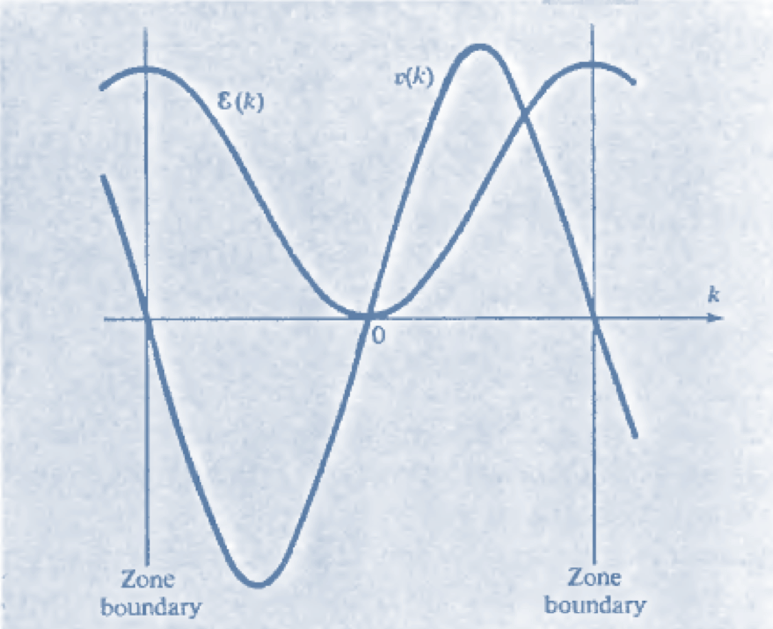
\includegraphics[width=0.8\textwidth]{figures/pzbv.png}
  \caption{Gráfica para la formulación semiclásica de la velocidad
    $\mathbf{v}_n = \nabla_\mathbf{k} \varepsilon$ en 1D. Se predicen oscilaciones
    electrónicas bajo un campo electrico constante debidas a la no
    linealidad de la energía.}
  \label{fig:pzbv}
\end{figure}

\subsection{Huecos}
Al ser la integral de $\mathbf{J}$ nula, podemos escribir
\begin{equation}
  \iiint_\text{all} \mathbf{v}(\mathbf{k}) \text{d}\mathbf{k} =
  0 = \iiint_\text{empty} \mathbf{v}(\mathbf{k})
  \text{d}\mathbf{k} + \iiint_\text{ocuppied} \mathbf{v}(\mathbf{k}) \text{d}\mathbf{k}
\end{equation}
Deduzco que puedo integrar sobre estados vacíos en lugar de estados
llenos sin más que cambiar el signo. Esta es la base del concepto de
\emph{hueco}; la ventaja está en que suele haber muchos menos estados
llenos y la integral es más fácil. Físicamente, consideramos
``huecos'' que se comportan como electrones de carga positiva.

Algunas de sus propiedades son (el subíndice \emph{h} denota a los
huecos y \emph{e} a los electrones):
\begin{enumerate}
\item $\mathbf{k}_h = - \mathbf{k}_e$
\item $\varepsilon_h (\mathbf{k}_h) = -\varepsilon_e (\mathbf{k}_e)$
\item $v_h = v_e$
\item $m_h = -m_e$
\item
  $\hbar \frac{\text{d}}{\text{d} t} \mathbf{k}_e = - e \left(
    \mathbf{E} + \nicefrac{1}{c}\ \mathbf{v}_e \times \mathbf{B}
  \right) \ \stackrel{k_h = -k_e}{\rightarrow} \ \hbar
  \frac{\text{d}}{\text{d} t} \mathbf{k}_h = - e \left( \mathbf{E} +
    \nicefrac{1}{c}\ \mathbf{v}_h \times \mathbf{B} \right)$
\end{enumerate}

\section{Movimiento en campos magnéticos}
Partimos de las ecuaciones semiclásicas del movimiento ya vistas, pero
suponiendo por simplicidad un campo eléctrico nulo:

\begin{equation}
\label{eq:sistemachungo}
  \begin{cases}
    \dot{ \mathbf{r} } &= \mathbf{v}_n(\mathbf{k}) = \dfrac{1}{\hbar} \nabla _\mathbf{k} \,
    \varepsilon_n (\mathbf{k}) \\
    \hbar \dot{\mathbf{k}} &= - e \mathbf{v}_n (\mathbf{k}) \times \mathbf{B}
  \end{cases}
\end{equation}
De la ecuación para $\mathbf{k}$ vemos que en el espacio recíproco el
electrón se mueve de manera perpendicular al gradiente de energía (hay
un producto vectorial), por lo que traza órbitas de energía constante,
moviéndose en superficies de $\varepsilon = \text{cte.}$

Si el electrón está en la superficie de Fermi (la cual es una
superficie de $\varepsilon = \text{cte.}$) se moverá en el plano
perpendicular al campo magnético, trazando órbitas abiertas o cerradas
según la superficie de Fermi corte o no a la primera zona de Brillouin
(fig. \ref{fig:fermiorbits}).

\begin{figure}
  \centering
  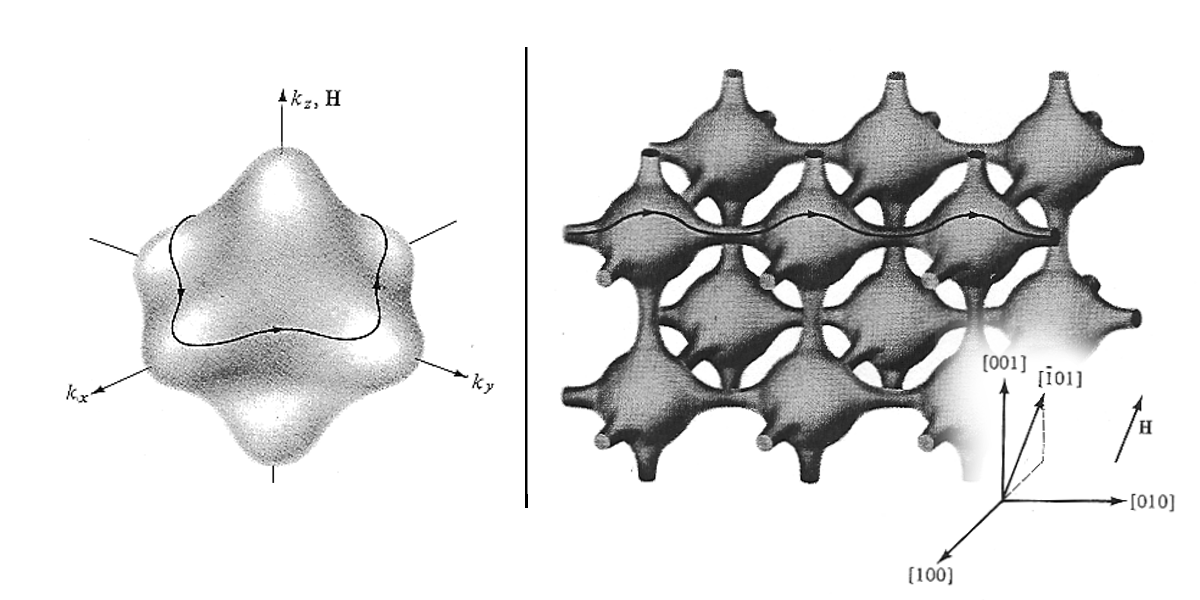
\includegraphics[width=0.8\textwidth]{figures/fermiorbits.png}
  \caption{Si la superficie de Fermi se sale de la primera zona de
    Brillouin se conecta con las de otras celdas unidad y la órbita es
    abierta (figura de la derecha). En caso contrario (figura de la
    izquierda) la órbita es cerrada.
    El sentido en que se recorre la órbita es contrario si estamos
    tratando con un hueco en lugar de un electrón. }
  \label{fig:fermiorbits}
\end{figure}

En el espacio real, las órbitas son iguales pero rotadas
$\nicefrac{\pi}{2}$ y escaladas, como se deduce de resolver (\ref{eq:sistemachungo}):
\begin{equation}
  \mathbf{r}_\perp (t) - \mathbf{r}_\perp (0) = \frac{-\hbar}{e B}
  \hat{B} \times (\mathbf{k}(t) - \mathbf{k}(0))
\end{equation}
La velocidad no es uniforme para una geometría arbitraria de la
superficie de energía constante.

podemos tratar de calcular el periodo de las órbitas. Imaginemos una
geometría como la de la figura \ref{fig:orbitgeom}.

\begin{figure}
  \centering
  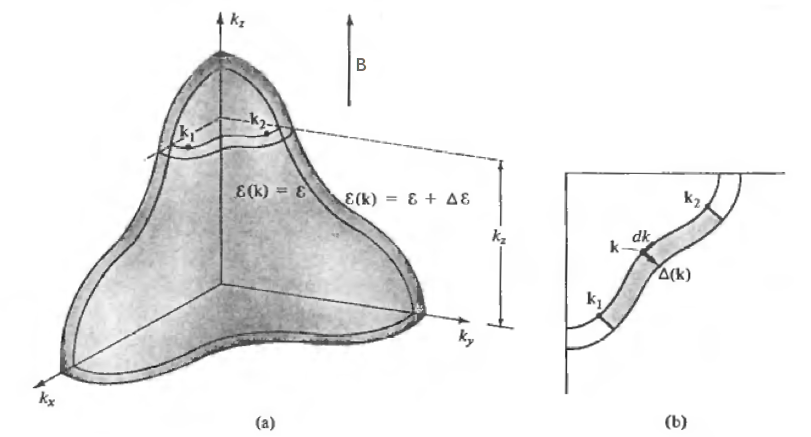
\includegraphics[width=0.8\textwidth]{figures/orbitgeom.png}
  \caption{(a) Geometría del problema tratado. Se tienen dos órbitas
    muy cercanas, con la misma $k_z$ pero distinta componente
    radial. El campo magnético externo $\mathbf{B}$ está en la
    dirección $k_z$. Las energías de ambas órbitas difieren en
    $\Delta \varepsilon$. (b) Se muestra también un corte transversal
    (plano $k_x, k_y$) en que se ve el vector
    $\boldsymbol{\Delta}(k) = \Delta \mathbf{k}$. El área sombreada
    corresponde a
    $\partial A_{1,2} / \partial \varepsilon \cdot \Delta
    \varepsilon$}
  \label{fig:orbitgeom}
\end{figure}

Suponemos un cambio del electrón de $\mathbf{k}_1$ a
$\mathbf{k}_2$. El cambio le cuesta un tiempo $\Delta t$:
\begin{equation}
  \Delta t = t_2 -t_1 = \int_{t_1}^{t_2} \text{d}t = \int_{t_2}^{t_1}
  \text{d}\mathbf{k}\  \left| \frac{\text{d}t}{\text{d}\mathbf{k}}
  \right| = \cdots
\end{equation}
Como $\dot{\mathbf{k}} = - \frac{e}{\hbar} \mathbf{v} \times
\mathbf{B}$ tenemos que $|\dot{\mathbf{k}}|^{-1} = \frac{\hbar}{evB}$,
    \begin{equation}
      \cdots =  \int_{\mathbf{k}_1}^{\mathbf{k}_2} \frac{\hbar}{eB}
      \frac{1}{\mathbf{v}_n(\mathbf{k})}\text{d}k =\frac{\hbar^2}{eB} \int_{\mathbf{k}_1}^{\mathbf{k}_2}
      \frac{1}{ \left| (\nabla_\mathbf{k}\varepsilon)_\perp\right|}\text{d}k = \cdots
    \end{equation}
donde la integral pasa a ser una integral de camino por
$\mathbf{k}(t)$. Usamos que la variación de energía entre dos $\mathbf{k}$ es $\Delta
\varepsilon = \Delta_\mathbf{k}\varepsilon\cdot\Delta \mathbf{k} =
|(\nabla_\mathbf{k}\varepsilon)_\perp|\cdot\Delta \mathbf{k}$ y
escribimos
\begin{equation}
  \cdots = \frac{\hbar^2}{eB} \int_{\mathbf{k}_1}^{\mathbf{k}_2}
  \frac{\Delta \mathbf{k}}{\Delta \varepsilon}\text{d}k = \cdots
\end{equation}

Tomando el límite $\Delta\varepsilon \to 0$,
\begin{equation}
  \cdots = \frac{\hbar^2}{eB} \frac{\int_{\mathbf{k}_1}^{\mathbf{k}_2}
  \Delta \mathbf{k} \ \text{d}k}{\Delta \varepsilon} =
\frac{\hbar^2}{eB} \pfrac{A_{1,2}}{\varepsilon}
\end{equation}

Si la órbita es cerrada $\mathbf{k}_1 = \mathbf{k}_2$ y $\delta t =
T$. Utilizando la fórmula clásica del ciclotrón despejamos la masa efectiva:
\begin{equation}
  T(\varepsilon, k_z) = \frac{\hbar^2}{eB} \frac{\partial}{\partial
    \varepsilon} A(\varepsilon,k_z) = \frac{2\pi}{eB}m^* (\varepsilon,k_z)
\end{equation}
Obtenemos la denominada \emph{masa efectiva ciclotrónica}:
\begin{equation}
  m^*_\text{cicl.}(\varepsilon,k_z) = \frac{\hbar^2}{2\pi}\frac{\partial}{\partial \varepsilon}A(\varepsilon,k_z)
\end{equation}
En el caso de electrones libres la energía es $\varepsilon =
\frac{h^2}{2m^*} k^2$ y $A$ no es más que el área de una
circunferencia, $A = \pi k^2$. En ese caso obtenemos que $m^*_\text{cicl.} = m^*$.

Si $m^* =m $ obtenemos
\begin{equation}
  T = \frac{2\pi}{\omega_c} = \frac{2\pi m}{eB} \ \rightarrow \
  f_c = \frac{\omega_c}{2\pi} = \frac{eB}{m} \stackrel{B = \SI{1}{\tesla}}{\sim} \SI{28}{\giga\hertz}
\end{equation}
\section{Niveles de Landau}
Nos restringimos a 2D por simplicidad (no hay pérdida de generalidad)
y consideramos el efecto de un campo magnético sobre un gas de
Fermi\footnote{No es necesario suponer electrones libres siempre y
  cuando la corrección esté completamente representada mediante una
  masa efectiva $m^*$.}. Sea un campo magnético $\mathbf{B} = B
\hat{k}$ sobre un gas de Fermi bidimensional en el plano $OXY$, el
hamiltoniano será:
\begin{equation}
  \mathcal{H} = \frac{1}{2m}(\mathbf{p} + e \mathbf{A})^2
\end{equation}
Es el del gas de Fermi corregido por el potencial vector
$\mathbf{A}$. Recordar que su elección no es única\footnote{La
  ecuación $\nabla \times \mathbf{A} = B \hat{k}$ tiene varias
  soluciones, como $(-By,0,0)^T$ o $\nicefrac{B}{2}(-y,x,0)^T$.}, esto tiene que ver
con la invariancia de gauge de la mecánica cuántica. Utilicemos el
\emph{gauge de Landau}, definido por $\mathbf{A} = Bx \hat{y}$. Se
tiene entonces que
\begin{equation}
  \begin{cases}
    (\mathbf{p}+e \mathbf{A}) &= (p_x,p_y + eBx,0)^T \\
    (\mathbf{p}+e \mathbf{A})^2 &= \cdots = p_x^2 + p_y^2 + (eBx)^2 +
    2p_y e Bx 
  \end{cases}
\end{equation}
y obtenemos para el hamiltoniano
\begin{equation}
  2m\mathcal{H} = 
    \underbrace{ p_x^2 + p_y^2}_{\mathcal{H}_0 \ \text{(free)}} +  \underbrace{(eBx)^2 +
    2p_y e Bx}_{\text{correction}}
\end{equation}
Aunque parezca un hamiltoniano muy complicado hay una simetría muy
importante: conmuta con $p_y$ ($[\mathcal{H},p_y] =0$).Con otros
gauges obtenemos relaciones de conmutación con otros
componentes.

Conocida esta relación de conmutación podemos ensayar una solución del
estilo de $\psi(x,y) = e^{i k_y y} u(x)$. Al sustituir en la ecuación
de Schrodinger independiente del tiempo ($\mathcal{H} \psi = E \psi$) obtengo
\begin{equation}
  \begin{split}
    - \hbar^2 \frac{\partial^2}{\partial x^2} u(x) + k_y ^2 \hbar^2
    u(x) + (eBx)^2 u(x) + 2eBx u(x)(-i \hbar i k_y) &= 2m E u(x) \\
    \left[ -\hbar^2 \frac{\partial^2}{\partial x^2} + k_y^2 \hbar^2 +
      (eBx)^2 + 2eBx \hbar k_y \right] u(x) &= 2m E u(x) \\
    \left[  -\hbar^2 \frac{\partial^2}{\partial x^2} + (k_y \hbar +
      eBx)^2 \right] u(x) = 2m E u(x)
  \end{split}
\end{equation}
Definiendo $x_0 = \frac{\hbar k_y}{eB}$ obtengo
\begin{equation}
  \left[  \frac{-\hbar^2}{2m} \frac{\partial^2}{\partial x^2} +
    \frac{1}{2m} eB (x+x_0)^2 \right] u(x) = E u(x)
\end{equation}
La ecuación tiene la forma de un oscilador armónico unidimensional con
$\omega = \frac{eB}{m}$ (la frecuencia de ciclotrón):
\begin{equation}
  \mathcal{H} =   \frac{-\hbar^2}{2m} \frac{\partial^2}{\partial x^2} +
    \frac{1}{2} m \omega^2 (x+x_0)^2 = \mathcal{H}_\text{osc}
\end{equation}
Las soluciones serán por tanto niveles discretos:
\begin{equation}
  E_n = \left( n + \frac{1}{2} \right) \hbar \omega_c \tag{Landau levels}
\end{equation}
Hemos pasado de un espectro de estados contínuo\footnote{Supuesto que
  el plano no estaba acotado. Las condiciones de contorno discretizan
  los niveles del gas de Fermi.} a uno discreto
(fig. \ref{fig:landaurings}). Los estados que teníamos se han
condensado en los anillos de Landau (no han podido desaparecer), lo
que hace que la degeneración de estos nuevos niveles no sea ni pequeña
ni trivial.

\begin{figure}
  \centering
  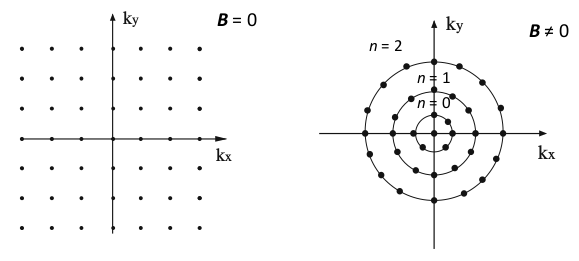
\includegraphics[width=0.8\textwidth]{figures/landaurings.png}
  \caption{Un campo magnético transversal a un gas de Fermi
    bidimensional discretiza sus posibles estados. }
  \label{fig:landaurings}
\end{figure}

\subsection{Degeneración de los anillos}
Las dimensiones del sistema vienen dadas por $L_x, L_y$; la imposición
de las condiciones de contorno periódicas resulta como ya se ha visto
en otras ocasiones en una discretización de los $k_y,k_x$:
\begin{equation}
  e^{ik_y y} =e^{ik_y
    (y+L_y)}  \rightarrow  e^{ik_y L_y} = 1  \rightarrow  k_y L_y
  = 2\pi m
\end{equation}
$k_y$ está también relacionado con $x_0$ vía $k_y = \frac{eB}{\hbar}
x_0$ este resulta también discretizado:
\begin{equation}
  x_0 = \frac{2\pi \hbar m}{eB L_y}
\end{equation}
Pero $x_0$ es un desplazamiento en la coordenada del oscilador
armónico, así que también está limitado por geometría ($x_0 \in
(0,L_x)$). Obtenemos una cota para $m$:
\begin{equation}
  m \in \left[ 0, \frac{e B L_x L_y}{2\pi \hbar} \right]
\end{equation}
La cota superior es la degeneración de los niveles de Landau,
$N_L$.
\begin{equation}
 m \in [0,N_L], \ \ N_L = \frac{eB S}{2\pi \hbar} 
\end{equation} 
Vemos que es proporcional a la superfice; esto era de esperar
porque cuanta más superficie en el espacio de momentos tenemos más
estados hay para aglutinar. También es proporcional al campo
magnético, lo que nos indica que al aumentarlo ``caben'' más estados
por anillo y se reduce su número.

\begin{boldproof}[Degeneración de los niveles de Landau]
Podemos comprobar la validez de $N_L$ contando el número de estados
entre dos anillos, $\pi(k_{n+1}^2 - k_n^2)\frac{L_x
  L_y}{4\pi^2}$. Contemplando el
espín\footnote{Añadir el espín implica tener en cuenta un término de
  interacción campo espín en el hamiltoniano, lo que provoca
  desdoblamiento de los anillos por efecto Zeeman. Por lo demás, la
  física es similar.} hay un dos en lugar de un cuatro en el
denominador; en este caso se prescindirá de el. Para cada anillo tenemos:
\begin{equation}
  \begin{cases}
    {\hbar^2 k_{n}^2}    &= 2m\hbar\omega_c (n + 1  ) \\
    {\hbar^2 k_{n+1}^2}  &= 2m\hbar\omega_c (n + 1 + \nicefrac{1}{2})
  \end{cases}
\end{equation}
El número de estados entre los anillos $n$ y $n+1$ resulta:
\begin{equation}
  \begin{split}
  N_n^{n+1} &=\pi(k_{n+1}^2 - k_n^2)\frac{L_x L_y}{4\pi^2} =  \pi (2m
  \hbar^{-1} \omega_c [n+1 + \nicefrac{1}{2} -n -1]) \frac{S}{4\pi^2}
  \\
  &= \frac{\omega_c m S}{2\pi \hbar} = \frac{eBS}{2\pi \hbar} = N_L
  \end{split}
\end{equation}
\end{boldproof}

Podemos escribir $N_L$ de manera alternativa:
\begin{equation}
  N_L = \frac{eB L_x L_y}{2 \pi\hbar} = \frac{\Phi}{\nicefrac{h}{e}} = \frac{\Phi}{\Phi_0}
\end{equation}
A $\Phi_0 \sim \SI{4.14e-7}{\gauss\per\centi\metre\squared}$ se le denota \emph{cuanto de flujo magnético}.

\subsection{Tratamiento general}
Visto el tratamiento de Landau nos planteamos si los resultados se
pueden extrapolar para un sólido, en el que los electrones no están
libres y hay una estructura de bandas superpuesta a posteriores
cuantizaciones. Para responder necesitaríamos repetir el análisis
contemplando en el hamiltoniano el potencial de bandas, pero eso es
muy complicado; en su lugar realizamos el tratamiento semiclásico
propuesto en 1956 por Onsager y Lifshitz, basado en la cuantificación
de Bohr-Sommerfield.

Partimos de
\begin{equation}
  \oint \mathbf{p} \text{d} \textbf{r} = (n + \gamma)2\pi \hbar
\end{equation}
donde el término $\gamma$ es una corrección a la fase de la función de
ondas sobre la condición de Bohr-Sommerfield original que vale
$\nicefrac{1}{2}$ para los electrones libres. Para el momento tenemos
que
\begin{equation}
  \mathbf{p} = \hbar \mathbf{k} -e \mathbf{A}
\end{equation}
donde el campo externo $\mathbf{B}$ queda representado mediante la
inclusión del potencial vector $\mathbf{A}$. Sustituyendo:
\begin{equation}
  \oint \textbf{p} \text{d}\textbf{r} = \oint \hbar \textbf{k} \text{d}r - e
  \oint \textbf{A} \text{d}\textbf{r}
\end{equation}
Hay que resolver dos integrales.
\begin{itemize}
\item Para la primera, utilizamos que $\hbar \dot{\textbf{k}} = -e \dot{\textbf{r}}\times
\textbf{B} \ \rightarrow \ \hbar \textbf{k} = -e \textbf{r} \times \textbf{B}$.
\begin{equation}
    \oint \text{d} \textbf{k} \text{d} \textbf{r }= -e \oint \textbf{r} \times \textbf{B} \text{d}
    \textbf{r} = e B \oint \textbf{r}\times
    \text{d}\textbf{r} = \cdots
\end{equation}
donde se ha usado que $(\textbf{A}\times \textbf{B})\cdot \textbf{C} =
(\textbf{C}\times \textbf{A})\cdot \textbf{B} = -
\textbf{B}(\textbf{A}\times \textbf{C})$ siendo
$\textbf{A}=\textbf{r}, \textbf{B} = \textbf{B}, \textbf{C} =
\text{d}\textbf{r}$. Utilizando que $\oint \textbf{r} \times
\text{d}\textbf{r} = 2A$, siendo $A$ el área encerrada en la órbita,
\begin{equation}
  \cdots = e B 2 A = 2e \Phi
\end{equation}
\item En la segunda integral se obtiene tras sustituir $\textbf{A} =
  \nabla \times \textbf{B}$:
  \begin{equation}
    -e \oint \textbf{A} \text{d}\textbf{r} = -e \oint \nabla \times
    \textbf{B} \text{d} \textbf{r} = -e \iint \textbf{B}
    \text{d}\textbf{A} = -e \Phi
  \end{equation}
  donde se ha utilizado el teorema de Stokes.
\end{itemize}
Se obtiene en definitiva
\begin{equation}
  \oint \textbf{p} \text{d}\textbf{r} = 2e \Phi - e \Phi = e \Phi =
  (n+\gamma)2\pi \hbar
\end{equation}
de manera que hemos recuperado la cuantificación del flujo de la
teoría de Landau sin suponer electrones libres:
\begin{equation}
  \Phi_n = (n + \gamma) \frac{h}{e} = (n+\gamma) \Phi_0
\end{equation}
\subsection{Oscilaciones}
Podemos analizar la relación de áreas en el espacio recíproco. Sea $A$
el área de una parcela del espacio real y $S$ la correspondiente en el
espacio recíproco correspondiente:
\begin{equation}
  \begin{split}
    \hbar \Delta k &= e \Delta r B \\
    \Delta r &= \frac{\hbar}{eB} \Delta k \\
    \underbrace{A}_{\text{m\textsuperscript 2}} &= \left(
      \frac{\hbar}{eB} \right)^2 \underbrace{S}_{\nicefrac{1}{\text{m
          \textsuperscript 2}}} \\
  \end{split}
\end{equation}

utilizando que $\Phi_n = (n+\gamma)  \nicefrac{h}{e}$ obtenemos
\begin{equation}
  \begin{split}
    \Phi_n &= B A_n = B \left( \frac{\hbar}{eB} \right)^2 S_n \\
     &= (n+\gamma) \frac{2\pi \hbar}{e}
  \end{split}
\end{equation}
y por tanto
\begin{equation}
  S_n = (n+\gamma) \frac{2\pi e B}{\hbar}
\end{equation}
Como en el modelo de Landau se obtiene una cuantificación de las áreas
barridas en el espacio recíproco, aunque se haya levantado la
restricción de electrones libres. Calculemos el incremento $\delta B$
necesario para que dos órbitas sucesivas $n,n+1$ tengan la misma área
$S$:
\begin{equation}
  \begin{cases}
    S_n &= S = (n+\gamma)\frac{2\pi e B_n}{\hbar} \\
    S_{n+1} &= S = (n+1+\gamma)\frac{2\pi e B_{n+1}}{\hbar}
  \end{cases} \ \rightarrow \ \frac{1}{B_{n+1}} - \frac{1}{B_n} =
  \Delta \left( \frac{1}{B} \right) = \frac{2\pi e}{\hbar S}
\end{equation}
La población de las órbitas en la superficie de Fermi
(y cercanas a ella) oscila con $B$, de forma que las propiedades
físicas experimentan diversas variaciones. Obtenemos que incrementos iguales de $\nicefrac{1}{B}$ producen las
mismas órbitas, por lo que estas variaciones en las propiedades
físicas mostrarán periodicidad en $\nicefrac{1}{B}$.

Históricamente, hay dos efectos de especial importancia:
\begin{description}
\item[Imanación] Las oscilaciones en la imanación de un metal al
  aplicar un campo magnético se denotan \emph{efecto de Haas-van
    Alphen} (efecto dHvA).
\item[Resistividad] A las oscilaciones en la magnetoresistencia se les

  \ref{fig:sdh} puede verse un ejemplo.
\end{description}

\begin{figure}
  \centering
  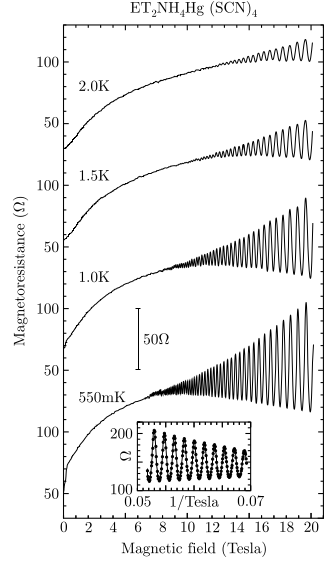
\includegraphics[width=0.5\textwidth]{figures/sdh.png}
  \caption{Las oscilaciones en la magnetoresistencia tienen
    periodicidad en $\nicefrac{1}{B}$, como puede verse en el inserto.}
  \label{fig:sdh}
\end{figure}
%%% Local Variables:
%%% mode: latex
%%% TeX-master: "../fesi.tex"
%%% End:
